%%%%%%%%%%%%%%%%%%%%%%%%%%%%%%%%%%%%%%%%%%%%%%%
%%% Template for lab reports used at STIMA
%%%%%%%%%%%%%%%%%%%%%%%%%%%%%%%%%%%%%%%%%%%%%%%

%% Sets the document class for the document
% Openany is added to remove the book style of starting every new chapter on an odd page (not needed for reports)
\documentclass[10pt, english, openany]{report}

%% Loading packages that alter the style
\usepackage[]{graphicx}
\usepackage[]{color}
\usepackage{alltt}
\usepackage[T1]{fontenc}
\usepackage[utf8]{inputenc}
\usepackage{textcomp}
\usepackage{hyperref}
\usepackage{amsmath}
\usepackage{multirow}
\usepackage{multicol}
\usepackage{colortbl}
\usepackage{color}
\usepackage[toc,page]{appendix}
\usepackage{subcaption}

\definecolor{Black}{rgb}{.0,.0,.0}

\setcounter{secnumdepth}{3}
\setcounter{tocdepth}{3}
\setlength{\parskip}{\smallskipamount}
\setlength{\parindent}{0pt}

% Set page margins
\usepackage[top=100pt,bottom=100pt,left=68pt,right=66pt]{geometry}

% Package used for placeholder text
\usepackage{lipsum}

% Prevents LaTeX from filling out a page to the bottom
\raggedbottom

% add English language
\usepackage[english]{babel}

% All page numbers positioned at the bottom of the page
\usepackage{fancyhdr}
\fancyhf{}                          % clear all header and footers
\fancyfoot[C]{\thepage}
\renewcommand{\headrulewidth}{0pt}  % remove the header rule
\pagestyle{fancy}

% Changes the style of chapter headings
\usepackage{titlesec}
\titleformat{\chapter}
{\normalfont\LARGE\bfseries}{\thechapter.}{1em}{}
% Change distance between chapter header and text
\titlespacing{\chapter}{0pt}{50pt}{2\baselineskip}

% Adds table captions above the table per default
\usepackage{float}
\floatstyle{plaintop}
\restylefloat{table}

% Adds space between caption and table
\usepackage[tableposition=top]{caption}

% Adds hyperlinks to references and ToC
\usepackage{hyperref}
\hypersetup{hidelinks, linkcolor = blue} % Changes the link color to black and hides the hideous red border that usually is created

% If multiple images are to be added, a folder (path) with all the images can be added here
\graphicspath{ {images/} }

% Separates the first part of the report/thesis in Roman numerals
%\frontmatter

%% USER Package
\usepackage{tabularx}
\usepackage{titling}

%% title2.tex
\title{Course Report of \\ Operational Research 2}
\author{Luca Perali 1237770 \\ Michele Thiella 1234567}
\date{\today}

%% Starts the document
\begin{document}

	%% Selects the language to be used for the first couple of pages
	\selectlanguage{english}

	%% Adds the title page
	
\begin{titlepage}
  \clearpage\thispagestyle{empty}
  \centering
  \vspace{2cm}

  % Titles
  
\includegraphics[scale=0.75]{uniLogo.png} \\ [1cm]
  \LARGE\textbf{University of Padua} \\ [4cm]
  \Huge\textbf{Travelling Salesman Problem} \\ [1cm]
  \Large\textbf{Course Report of \\ Operational Research 2} \\ [4cm]
  \begin{table}[h]
    \begin{tabularx}{\textwidth}{X r}

        \Large\textit{Professor}  & \Large\textit{Author, ID number} \\ [0.2cm]
        \Large\textsc{Matteo Fischetti}  & \Large\textsc{Luca Perali, 1237770} \\ [0.2cm]
          & \Large\textsc{Michele Thiella } \\ [0.3cm]
        \hline
    \end{tabularx}
  \end{table}

  % Set the date
  \textsc\Large \today \\ [2cm]

  \pagebreak
\end{titlepage}

	
\begin{abstract}
  this is the abstract
\end{abstract}


	% Adds a table of contents
	\tableofcontents{}
	\clearpage

	%%%%
	%% The rows above should not be changed except for the title page information
	%%%% Text body starts here!
	%\mainmatter
	\chapter{Problem description}
\label{chapter:TSPdescription}
\begin{figure}[h]
	\centering
	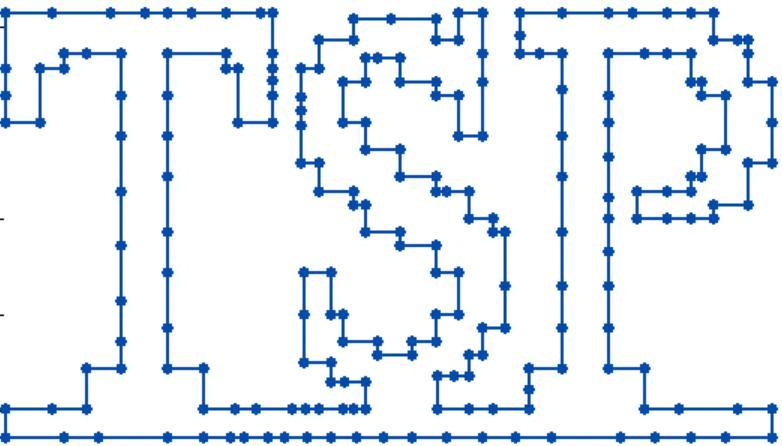
\includegraphics[width=.5\columnwidth]{img/tsp225_plot}
	\caption{The \textit{tsp225.tsp} instance from \textit{tsplib} resolved with \texttt{subtour} method described in cap \ref{sec:subtour} plotted with Gnuplot.}
	\label{fig:tsp225}
\end{figure}

The Traveling Salesman Problem is a well-known NP-hard problem. In short, given a set of cities it's required to find the shortest tour that visit exactly one time each city and return to the first one.
In this report two version of the TSP will be analyzed in details:
\begin{itemize}
	\item symmetric TSP (sTSP): with bidirectional edges;
 	\item asymmetric TSP (aTSP): with oriented arcs.
\end{itemize}


\section{Symmetric TSP}

\begin{figure}[h]
	\centering
	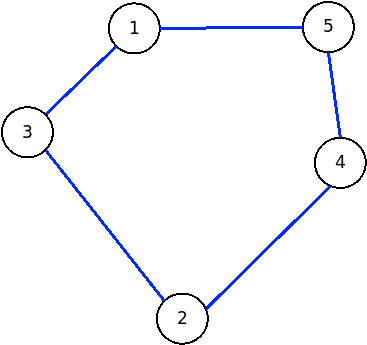
\includegraphics[width=.3\columnwidth]{img/symTSP_example.png}
	\caption{Example of tour. Only the selected edges are visible.}
	\label{fig:symTSP}
\end{figure}

Given a complete graph $ G = (V, E) $, a distance function $ d $ where:
\begin{itemize}
	\item $ V := \{1, 2, .., n\}$ is a set of nodes;
	\item $ E $ is the set of edges between each node pairs $ i,j \in V, i \ne j $ represented with $ (i,j) $ or for a generic edge $ e $, note that for sTSP $ (i,j) = (j,i) $ therefore the number of edges $ |E| = \frac{n(n-1)}{2} $;
	\item $ d: (i,j) = e \to d(i,j) = c_e $ where $ c_e $ is the cost associated to $ e \in E $;
\end{itemize}
and defining the decision variable:
\[
x_e := \begin{cases}
	1 & \text{if $ e $ is in the tour,} \\
	0 & \text{otherwise}
\end{cases}
\] 
the sTSP can be represented with linear programming system in \ref{eq:sTSP_LP}. 
\begin{equation}
\begin{cases}
		min \sum_{ e\in E } c_ex_e & \text{Cost function} \\
		\sum_{e\in \delta (v) } x_e = 2, \forall v \in V  & \text{Degree constraint} \\
		\sum_{e\in E(S) } x_e \le |S|-1, \forall S \subset V, |S| \ge 3  & \text{Subtour elimination} \\
		x_e \in \{0,1\}, \forall e \in E & \text{Domain constraint}
\end{cases}
\label{eq:sTSP_LP}
\end{equation} 
As usual it is required to find the value of $ x_e, \forall e \in E $ that minimize the \textit{cost function} and verify the constraints.
For the \textit{degree constrain}, the degree of each $ v \in V $ ($ |\delta(v)| $) must be equal to 2. A system with only the degree constrain (and the domain constraint) would probably have a set of subtours with size three or more, however by adding the \textit{subtour elimination} constraints  it's impose to have only one tour.

The number of possible subset $ S \subset V $ is exponential ($ 2^{n} - \binom{n}{3} -\binom{n}{2} -\binom{n}{1} - 1 = O(2^n)$), therefore even a graph with 100 nodes has huge matrix dimension. Note that $ E(S) := \{ e = (i,j): i,j \in S \subset V \}$ is the set of edges with both vertices in $ S $.\\
Considering the example in fig. \ref{fig:symTSP}, the value of the solution is represented in the matrix in tab. \ref{tab:symTSP_solution} where $ x_{ij} = x_{ji} $ for each $ i,j \in V, i \ne j $ but only the cell with $ i < j $ have been completed to enhance the number of variables that are used in practice.

\begin{table}[h!]
	\begin{center}
		\caption{Decision variable matrix. It show the value $ x_{ij} $ of the solution represented in figure \ref{fig:symTSP}. Due to the symmetry of the matrix, only the cell with $ i < j $ have a value, the others can be checked from the first.}
		\label{tab:symTSP_solution}
		\begin{tabular}{cc|c|c|c|c|c|}
			 \multicolumn{2}{c}{} & \multicolumn{5}{c}{j} \\ % <-- Combining two cells with alignment c| and content 12.
			& \multicolumn{1}{c}{} & \multicolumn{1}{c}{1} & \multicolumn{1}{c}{2} & \multicolumn{1}{c}{3} & \multicolumn{1}{c}{4} & \multicolumn{1}{c}{5} \\ \cline{3-7}
			\multirow{5}{*}{i} 	& 1 & \cellcolor{Black} & 0 & 1 & 0 & 1 \\ \cline{3-7}
								& 2 &  & \cellcolor{Black} & 1 & 1 & 0 \\ \cline{3-7}
								& 3 &  &  & \cellcolor{Black} & 0 & 0 \\ \cline{3-7}
								& 4 &  &  &  & \cellcolor{Black} & 1 \\ \cline{3-7}
								& 5 &  &  &  &  & \cellcolor{Black} \\ \cline{3-7}
		\end{tabular}
	\end{center}
\end{table}



\section{Asymmetric TSP}
Given a complete graph $ G = (V,A) $, a distance funciton  $ d $ where:
\begin{itemize}
	\item $ V:= \{1, 2, .., n\} $ is the set of nodes;
	\item $ A := $ the set arcs between each nodes $ i,j \in V, i \ne j$ represented as $ (i,j) $, note that in the aTSP $ (i,j) \ne (j,i) $ and the number of arcs is $ |A| = n (n-1) $ which is double of the sTSP;
	\item $ d: (i,j) \rightarrow d(i,j) = c_{ij} $ where $ c_{ij} $ is the cost associated to the arc $ (i,j) $.
\end{itemize}
As in the sTSP, it is defined the decision variable $ x_{ij} $ which tell if the arc $ (i,j) $ is in the tour:
\[
x_{ij} := \begin{cases}
1 & \text{if $ (i,j) $ is in the tour,} \\
0 & \text{otherwise}
\end{cases}
\]

The aTSP can be defined in different ways, in this report two version will be considered in detail: Miller Tucker Zemlin \cite{miller1960integer} and Flow1 by Gavish and Graves \cite{gavish1978travelling}.


\subsection{Miller Tucker Zemlin}

\begin{figure}[h]
	\centering
	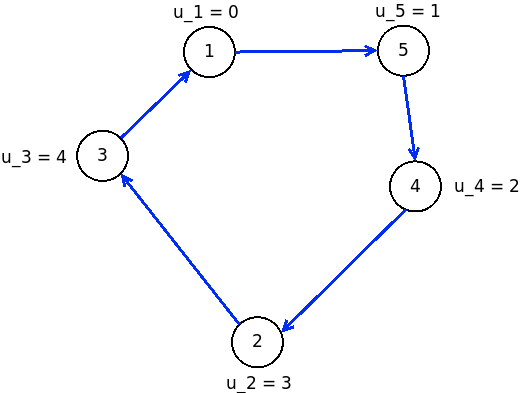
\includegraphics[width=.45\columnwidth]{img/asymTSP_MTZ_example.png}
	\caption{Example of tour with MTZ model. Only the selected arcs are visible and for each node $ k $, the decision variable $ u_k $ represent the posizion of the node in the tour.}
	\label{fig:asymTSP_MTZ}
\end{figure}

Miller Tucker Zemlin (MTZ) model impose the "subtour elimination" constraints with the help of another decision variable $ u_k $. For each node $ k = 2,..,n $, $ u_k $ is the position of the node $ k $ in the tour that start from the node $ 1 $. As an example in fig \ref{fig:asymTSP_MTZ} it is shown that $ u_1 = 0 $ and than $ u_k $ increase until $ n-1 $ along the tour.

The proposed model is shown in the system of equations \ref{eq:aTSP_MTZ}. The cost function and the degree constraints are adapted to the asymmetric problem, moreover MTZ constraint is derived from $ u_j \ge u_i+1-M(1-x_{ij}), \forall i,j \in V \backslash \{1\}, M \gg 0 $. Considering an arc $ (i,j) \in A \backslash \{1\} $, if it is in the tour then $ u_j \ge u_i + 1 $ because $ M(1-x_{ij}) = 0 $, else $ u_j \ge u_i + 1 - M < 0 \implies u_j \ge 0 $. For example for the arc $ (4,2) $ in fig \ref{fig:asymTSP_MTZ}, $ 3 \ge 2 + 1 - M(1-1) \iff 3 \ge 3 $. \\
Note that, if the value of M is less than $|V| - 1$  then the constraint is incorrect, otherwise a value of M greater than $|V| - 1 $ makes the constraint redundant, therefore the best value of M is $|V| - 1$, as implemented. \\
\begin{equation}
\begin{cases}
min \sum_{i\in V}\sum_{j\in V} c_{ij}x_{ij} & \text{Cost function} \\
\sum_{i\in V} x_{ih} = 1, \forall h \in V  & \text{$ x $ Outer arcs degree} \\
\sum_{i\in V} x_{hi} = 1, \forall h \in V  & \text{$ x $ Inner arcs degree} \\
u_i -u_j +M x_{ij} \le M - 1, \forall i,j \in V \backslash \{1\} & \text{MTZ constraints ($ O(n^2) $)} \\
0 \le x_{ij} \le 1, Integer, \forall i,j \in N  & \text{$ x $ Domain} \\
0 \le x_{ii} \le 0, Integer, \forall i \in N  & \text{} \\
0 \le u_{i} \le n-2, Integer, \forall i \in N \backslash \{1\} & \text{$ u $ Domain} 
\end{cases}
\label{eq:aTSP_MTZ}
\end{equation}


Note that the number of MTZ constraints is $ O(n^2) $, one for each arc, therefore much less respect sTSP model.\\
The number of decision variables instead is more than the double $ n(n-1) + n = n^2 $. Computational consideration will be done in the next chapter.

\begin{table}[h!]
	\begin{center}$  $
		\caption{Decision variable matrix. It show the value $ x_{ij} $ and $ u_k $ of the solution represented in figure \ref{fig:asymTSP_MTZ}. }
		\label{tab:asymTSP_MTZ_solution}
		\begin{tabular}{cc|c|c|c|c|c|}
			 $ x_{ij} $ & \multicolumn{1}{c}{} & \multicolumn{5}{c}{j} \\ % <-- Combining two cells with alignment c| and content 12.
			& \multicolumn{1}{c}{} & \multicolumn{1}{c}{1} & \multicolumn{1}{c}{2} & \multicolumn{1}{c}{3} & \multicolumn{1}{c}{4} & \multicolumn{1}{c}{5} \\ \cline{3-7}
			\multirow{5}{*}{i} 	& 1 & \cellcolor{Black} & 0 & 0 & 0 & 1 \\ \cline{3-7}
			& 2 & 0 & \cellcolor{Black} & 1 & 0 & 0 \\ \cline{3-7}
			& 3 & 1 & 0 & \cellcolor{Black} & 0 & 0 \\ \cline{3-7}
			& 4 & 0 & 1 & 0 & \cellcolor{Black} & 0 \\ \cline{3-7}
			& 5 & 0 & 0 & 0 & 1 & \cellcolor{Black} \\ \cline{3-7}
			\multicolumn{7}{c}{} \\ 
			
			\multicolumn{2}{c}{} & \multicolumn{5}{c}{$ k $} \\  
			& \multicolumn{1}{c}{} & \multicolumn{1}{c}{1} & \multicolumn{1}{c}{2} & \multicolumn{1}{c}{3} & \multicolumn{1}{c}{4} & \multicolumn{1}{c}{5} \\ \cline{3-7}
 			$ u_k $ &  & 0 & 3 & 4 & 2 & 1 \\ \cline{3-7}
		\end{tabular}
	\end{center}
\end{table}

\subsection{Flow1}

\begin{figure}[h]
	\centering
	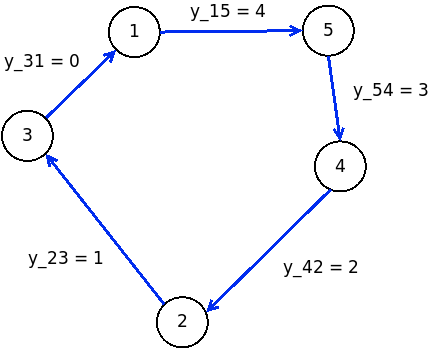
\includegraphics[width=.4\columnwidth]{img/asymTSP_F1_example.png}
	\caption{Example of tour with Flow1 model. Only the selected arcs are visible. $ y_{ij} $ is the decision variable that represent the decreasing flow of each arcs of the tour. Note that $ y_{ij} = 0 $ for each unselected arcs and in the figure they are not shown.}
	\label{fig:asymTSP_F1}
\end{figure}

The Flow1 model impose the "subtour elimination" constraints with a decision variable $ y_{ij} $ which is associated to each arc $ (i,j) \in V $ and represent a flow that decrease from $ n-1 $ to $ 0 $ for each node of the tour and is $ 0 $ if it is not in the tour. As shown in fig \ref{fig:asymTSP_F1} starting from the node $ 1 $ the flow $ y_{15} = 4 $ than decrease each step by $ 1 $ unit until the last arc of the tour where $ y_{31} = 0 $. Note that the last arc $ y_{31} $ has the same value of the unselected one, this is because the last arc of the tour is implicit. \\
The proposed LP model is in the system of equations \ref{eq:aTSP_F1}. The outer flow of $ 1 $ is the first constraint, than to make the flow decrease it is imposed the "flow equilibrium" where each inner flow must be equal to the outer flow $ +1 $ and, in the end, the \textit{coupling constraints} imposed that only the arcs in the tour ($ x_{ij} > 0 $) can have $ y_{ij} > 0 $ otherwise must be equal to $ 0 $. The last set of constraint force the flow to move along the tour and decrease each step. 

\begin{equation}
\begin{cases}
min \sum_{i\in V}\sum_{j\in V} c_{ij}x_{ij}  & \text{Cost function} \\
\sum_{i\in V} x_{ih} = 1, \forall h \in V  & \text{$ x $ Outer arcs} \\
\sum_{i\in V} x_{hi} = 1, \forall h \in V  & \text{$ x $ Inner arcs} \\
\sum_{j\in V} y_{1j} = n-1  & \text{$ 1 $ Outer flow} \\
\sum_{j\in V} y_{hj} = \sum_{i \in V}y_{ih} - 1, \forall h \in V \backslash \{1\}  & \text{Flow equilibrium} \\
y_{ij} - x_{ij}(n-1) \le 0, \forall i \in V, \forall j \in V \backslash \{1\}  & \text{Coupling constraints} \\
0 \le x_{ij} \le 1, Integer, \forall i,j \in N  & \text{$ x $ Domain} \\
0 \le x_{ii} \le 0, Integer, \forall i \in N & \text{} \\
0 \le y_{i1} \le 0, \forall i \in V  & \text{$ y $ Domain} \\
0 \le y_{ii} \le 0, \forall i \in V  & \text{} \\
0 \le y_{ij} \le n-1, Integer, \forall i,j \in V  & \text{} 
\end{cases}
\label{eq:aTSP_F1}
\end{equation}


The number of F1 constraint is equal to $ O(1) + O(n-1) + O(n^2) = O(n^2) $. The tables of variable are shown in tab \ref{tab:asymTSP_F1_solution} with the associated solution example in fig \ref{fig:asymTSP_F1}. It's easy to see that the number of variable is $ 2n(n-1) = O(n^2) $\\


\begin{table}[h!]
	\begin{center}
		\caption{Decision variable matrix. It show the value $ x_{ij}, y_{ij} $ of the solution represented in figure \ref{fig:asymTSP_F1}.}
		\label{tab:asymTSP_F1_solution}
		\begin{tabular}{cc|c|c|c|c|c|}
			
$ x_{ij} $ & \multicolumn{1}{c}{} & \multicolumn{5}{c}{j} \\ % <-- Combining two cells with alignment c| and content 12.
& \multicolumn{1}{c}{} & \multicolumn{1}{c}{1} & \multicolumn{1}{c}{2} & \multicolumn{1}{c}{3} & \multicolumn{1}{c}{4} & \multicolumn{1}{c}{5} \\ \cline{3-7}
\multirow{5}{*}{i} 	& 1 & \cellcolor{Black} & 0 & 0 & 0 & 1 \\ \cline{3-7}
& 2 & 0 & \cellcolor{Black} & 1 & 0 & 0 \\ \cline{3-7}
& 3 & 1 & 0 & \cellcolor{Black} & 0 & 0 \\ \cline{3-7}
& 4 & 0 & 1 & 0 & \cellcolor{Black} & 0 \\ \cline{3-7}
& 5 & 0 & 0 & 0 & 1 & \cellcolor{Black} \\ \cline{3-7}
\multicolumn{7}{c}{} \\ 

$ y_{ij} $ & \multicolumn{1}{c}{} & \multicolumn{5}{c}{j} \\ % <-- Combining two cells with alignment c| and content 12.
& \multicolumn{1}{c}{} & \multicolumn{1}{c}{1} & \multicolumn{1}{c}{2} & \multicolumn{1}{c}{3} & \multicolumn{1}{c}{4} & \multicolumn{1}{c}{5} \\ \cline{3-7}
\multirow{5}{*}{i} 	& 1 & \cellcolor{Black} & 0 & 0 & 0 & 4 \\ \cline{3-7}
					& 2 & 0 & \cellcolor{Black} & 0 & 0 & 0 \\ \cline{3-7}
					& 3 & 1 & 0 & \cellcolor{Black} & 0 & 0 \\ \cline{3-7}
					& 4 & 0 & 2 & 0 & \cellcolor{Black} & 0 \\ \cline{3-7}
					& 5 & 0 & 0 & 0 & 3 & \cellcolor{Black} \\ \cline{3-7}
			
		\end{tabular}
	\end{center}
\end{table}
	\chapter{CPLEX implementation and performance}

\section{CPLEX}
IBM ILOG CPLEX Optimizer is a solver licensed software, part of the IBM ILOG Optimizer Studio, with high level of efficiency and robustness \cite{IBMILOGCPLEX}. It can resolve a wide variety of problems:
\begin{itemize}
	\item Linear Programming (LP)
	\item Network Flow,
	\item Quadratic Programming (QP),
	\item Quadratically Constrained Programming (QCP),
	\item Mixed Integer Programming (MIP).
\end{itemize}
The interest, for the course purposes, is the LP optimization used to solve the TSP problem. The library written in C language, allow to define and resolve LP models with different heuristics and exact algorithm. The challenge is to implement with a state of the art LP solver the models specified in the chapter \ref{chapter:TSPdescription}, comparing time performance. 

\subsection{Callback}
\subsubsection{Lazy callback}
\subsubsection{Generic callback}



\section{Subtour Elimination}\label{sec:subtour}
The subtour elimination model described above enhance an exponential number of constraint ($ O(2^n) $), therefore it is not practicable to insert all the constraint in the model definition, instead is preferable to resolve the continuous relaxation without subtour elimination and than check if the solution verify the constraints, otherwise add the more violated constraints to the model. Four different version of subtour elimination model has been created:
\begin{enumerate}
	\item \textit{subtour\_iter\_opt}: the iteration apply the optimization step (\textit{CPX\_mipopt()}) and externally check the subtour constraints and eventually add the violated to the model. When no constraint is violated the best solution is found.
	\item \textit{subtour\_heur\_iter\_opt}: is equal to the previous one, but for the first iteration the subtour check is done immediately after the first available solution is found.
	\item \textit{subtour\_callback\_lazy}: While in the first two method the check is done outside CPLEX, here are used the \textit{CPXaddlazyconstraints()} which allow to check the constraints each time an incumbent should be update and to add the violated ones.
	\item \textit{subtour\_callback\_general}: The \textit{CPXcallbacksetfunc()} allow to set up a callback specifying the context in which to call that function. In this method is used to apply the lazy constraint with \textit{CPXcutcallbackadd()} in the \textit{CPX\_CALLBACKCONTEXT\_CANDIDATE} context.
\end{enumerate} 

\begin{figure}[h]
	\begin{subfigure}{.5\textwidth}
		\centering
		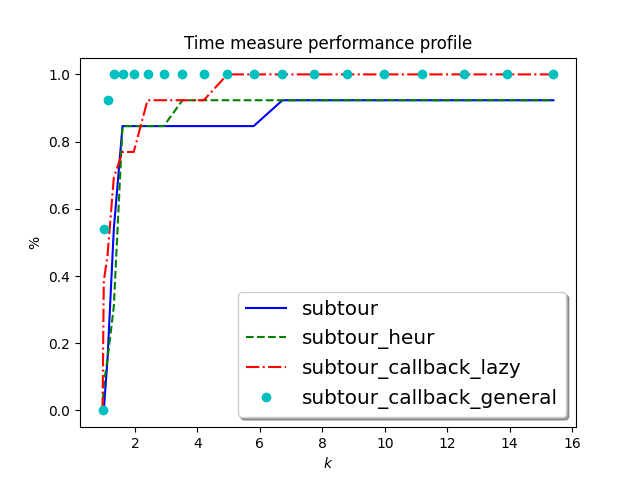
\includegraphics[width=\columnwidth]{../res/Lsubtours_average_time.png}
		\caption{Performance profile of the Data Average set}
		\label{fig:res_subtour_av}
	\end{subfigure}
	\begin{subfigure}{.5\textwidth}
	\centering
	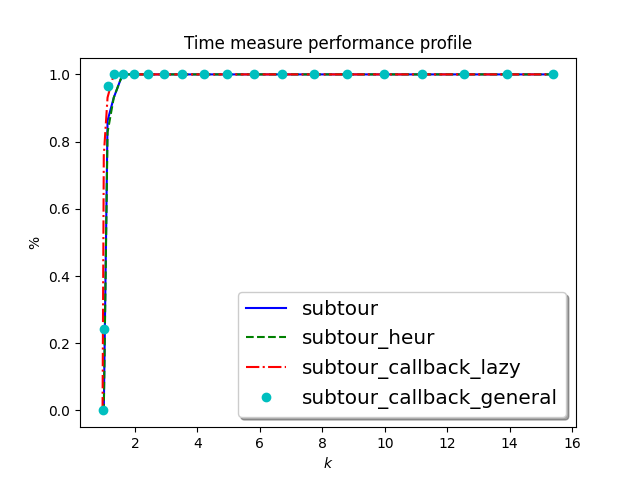
\includegraphics[width=\columnwidth]{../res/Lsubtours_light_time.png}
	\caption{Performance profile of the Data Light set}
	\label{fig:res_subtour_li}
	\end{subfigure}
\end{figure}

The performance profile in figure \ref{fig:res_subtour_av} is obtained by executing each subtour method in each Data Average instance for 5 different random seed generator. It show that in the $ 80\%  $  of the instances the \textit{subtour\_callback\_general} perform better than the other 3 alternatives.

qualche ulteriore dettaglio implementativo

confronto tra user callback e generic callback 

performance profile


\section{Miller Tucker Zemlin}

considerazioni sul numero di vincoli e sul problema asimmetrico

dettagli implementativi


\section{Flow Chart}

considerazioni sul numero di vincoli e sul problema asimmetrico

dettagli implementativi

performance profile con MTZ

	\chapter{Concorde TSP Solver}

	\chapter{Meta-heuristics}

\section{Hard-fixing}
A simple idea to reduce the complexity of the problem is to get an initial solution link an incumbent, fix some active edges and resolve the subproblem with CPLEX. This is exactly the idea behind hard fix approach.\\
The implementation proposed is applied in STSP problem, with the optimization of the general callback (\textit{subtour\_callback\_general}).
The algorithm can be divided in step:
\begin{enumerate}
	\item calculate an initial solution: in our implementation this is calculated by CPLEX with the \textit{subtour\_callback\_general} and \texttt{CPX\_PARAM\_INTSOLLIM} set to 1. When the first incumbent is available,the optimization terminate and a solution is obtained.
	\item fix a percentage of edges (fixing rate $ f_r $): edges are fixed using \texttt{CPXchgbds()} method that change the upper and lower bound of the decision variables. The fixing percentage is an important parameter: fixing too much edges leads to a fast resolution of the subproblem however increase the risk of obtaining the same solution and fall in a loop. Fixing too low edges involves slower resolution. In the first iteration $ f_r = 0.9 $.
	\item CPLEX optimization with time limit: After the fixing phase, the problem is optimized with \texttt{CPX\_mipopt()} and a short time limit is set ($ = 50 $s).
	\item fixing rate update: after the last phase, if the returned solution is improved better than a fixed gap ($  good\_gap $), it is considered a good solution and the $ f_r $ is increased by a constant ($ incr\_f_r $) until a max ($ max\_f_r $) otherwise if the new solution is not increased enough (less than $ optimal\_gap $), $ f_r $ is decreased of a constant ($ decr\_f_r $) until a min ($ min\_f_r $). Note that $ good\_gap $ and $ optimal\_gap $ are expressed as fraction of the best lower bound.
	\item check end condition: if the time limit is reached, or $ f_r = 0.0 $ and the solution is not improved in the last iteration then the solution is returned. Note that in the second case, the best solution is found. In case that no ending condition is satisfy, the algorithm continue with point 3.
\end{enumerate}

The performance profile as shown in fig \ref{fig:Lsubtours_hardfixing_lightaverage_time}. Hard fixing has performance comparable with the exact model.

\begin{figure}[h]
	\centering
	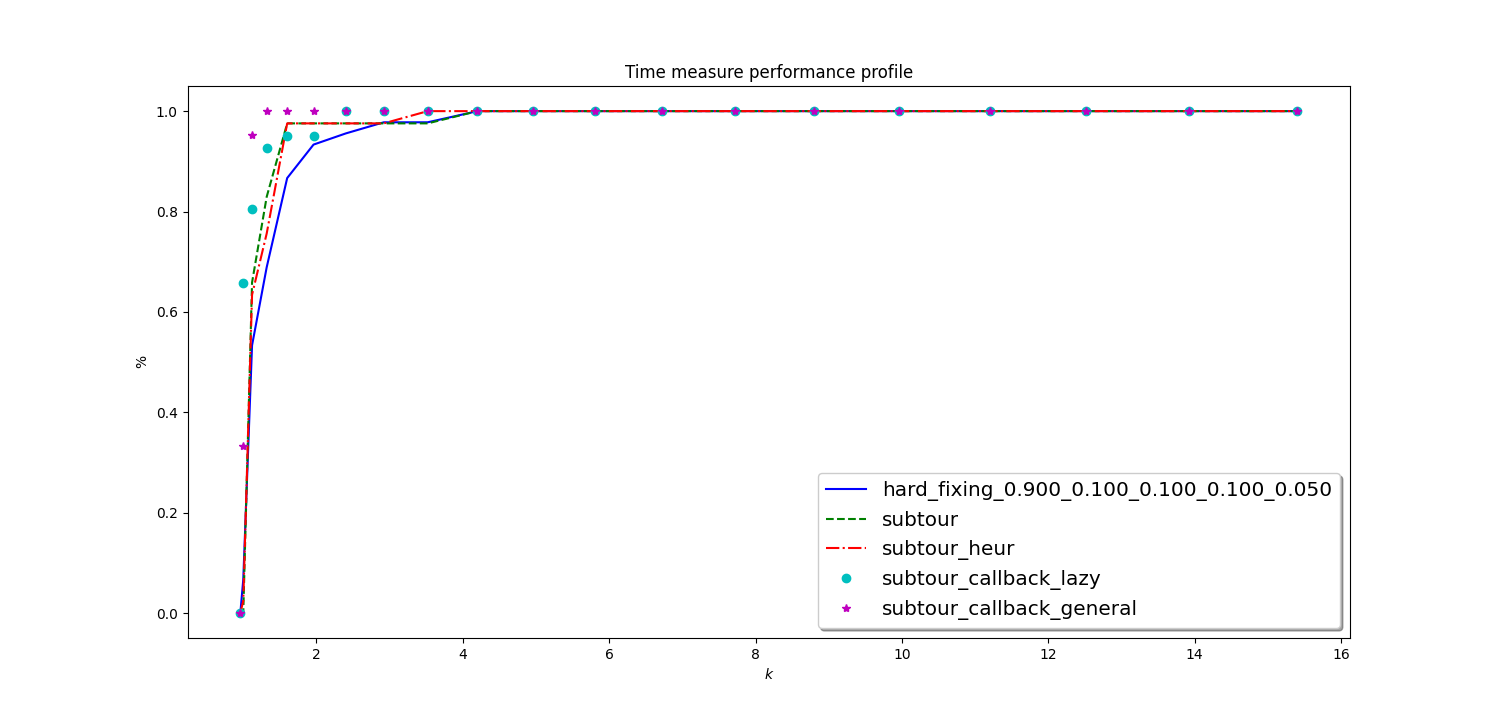
\includegraphics[width=\columnwidth]{../res/Lsubtours_hardfixing_lightaverage_time.png}
	\caption{Performance profile to compare subtours methods with \textit{hard\_fixing}. The name of \textit{hard\_fix} model contain in order: $ max\_f_r, incr_fr, decr\_f_r, good\_gap, optimal\_gap $. The test set is the composition of data\_light and data\_average.}
	\label{fig:Lsubtours_hardfixing_lightaverage_time}
\end{figure}


\section{Local-Branching}

\section{Tabu-Search}
Tabu Search (TS) has been developed by Fred Glover \cite{Glover1998}. TS is a heuristic that combines a local search process with a number of anti-cycling rules which prevent the search from getting trapped in a local minimum. Tabu Search is very similar to a local search algorithm that proceeds iteratively from one solution to another through the Best-2-opt \ref{sec:best_2_opt} method. It also uses a special memory structure, called a tabu list, that determines which subsequent solution will be chosen and therefore to organize the way space is explored. The algorithm starts with a random solution. By applying the Best-2-opt, as long as a new improvement solution is found, it updates the current solution to it. When it comes to a local minimum (i.e. there are no improvement solutions around two optimality) the use of the tabu list comes into play.\\
Pejorative moves are now allowed and the algorithm chooses the lowest cost one and adds this move to the tabu list, updates the current solution and starts again with the Best-2-opt.
During the next iteration, while searching for the new solution, check that the move to obtain it does not belong to the list. If it does not appear, then the move is lawful and continues with the next steps of the algorithm. Conversely, if the move is tabu (i.e. not allowed, prohibited), the solution is discarded and another is chosen, until a lawful move is found. The algorithm will continue to choose licit pejorative moves until an improvement one, that does not belong to the list, is found. In this case the algorithm starts again.\\
As will be discussed later, the tabu list has a maximum size of elements. Consequently, when a new element has to be inserted and the list is full, the "oldest" element (i.e. the one that has been inserted longer) of the list will be replaced with it.\\
This strategy allows research to move along the "hills" that the costs of the various solutions form in the solution space. It is an excellent method to escape from the local minimum by maintaining a search based on the Best-2-opt (Figure \ref{fig:tabu_search_perform_time}).\\
Looking at the implementation details there are many aspects that must be carefully evaluated:

\begin{itemize}
\item Type of structure for tabu list
\item Size of tabu list
\item Termination criterion
\end{itemize}

First of all, the type of structure used for the tabu list. We have decided to propose two different solutions, as each of them has its potential and its defects. The first, more classic, involves the use of a fixed-size array to store prohibited moves (so for each Best-2-opt move, the two relative edges are inserted into the array). The second, however, uses a linked list in which each element is formed by a variable for the edge and a pointer \textit{next} to the next element.
One of the main differences is the allocation of memory, as the linked list dynamically manages its size and therefore aims to optimize space but, on the other hand, the removal of the oldest inserted element requires complete scrolling of the list. Instead the array optimizes the operations on the elements contained but on the other hand it cannot have a dynamic dimension except through the creation and the copy in a new array (probably with an excellent knowledge of low-level memory and an ad hoc solution is possible to manage dynamic dimension of an array). For the management of the elements in the array it was decided to add one more element than the value of the chosen dimension, assigning it a static value of -1 that will never be changed. In this way, replacing an element when the list is full is very simple as it is sufficient to assign the new edge instead of -1 and replace the next element with -1. This causes the array to be cyclical and, through a single index variable, does not require any research for this type of operation.\\
Another aspect to consider is the size of the tabu list. An "infinite" dimension would risk bringing the algorithm to a standstill in which it can no longer make any move since all those around two optimality have been prohibited. Conversely, too small a size could cause a return to the local minimum from which one was running away. A lot of studies and research have been done for this specific aspect \cite{Nababan_2019, Tsubakitani1998} and a better overall result than others has not been found, changing the typology of the problem also varies the best size of the list. An average list size with respect to the problem proved to be the best choice as a balance between computational time and the optimal markspace value. Thus a size equal to half the number of problem nodes was set.\\
Finally, the termination criterion can be based on a maximum number of iterations of the algorithm or on a fixed number of iterations in which the solution no longer improves or, as in our case, on a timelimit.

\begin{figure}[h]
	\centering
	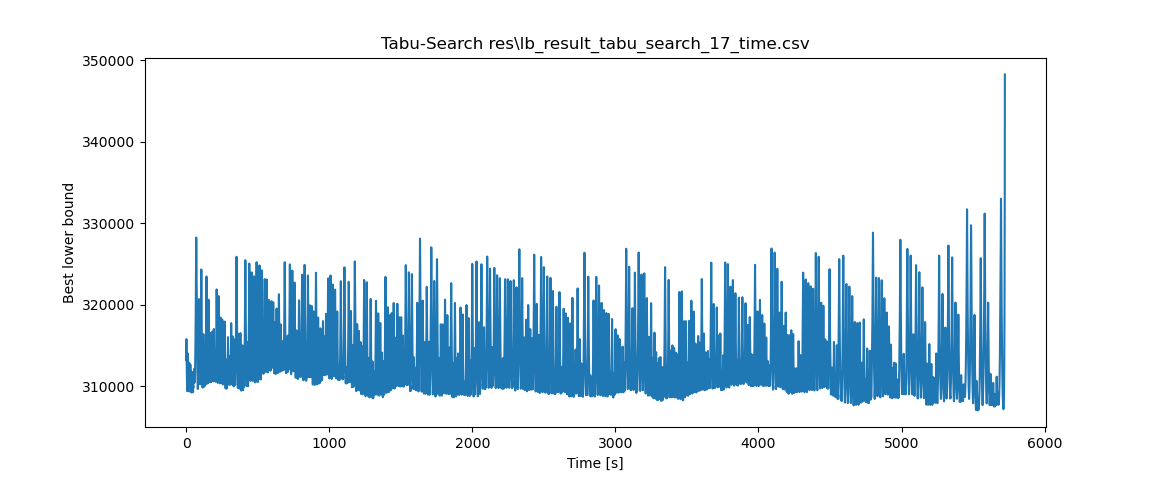
\includegraphics[width=1.0\columnwidth]{../res/gr666_17.png}
	\caption{Performance profile considering the execution time}
	\label{fig:tabu_search_perform_time}
\end{figure}

\section{Simulated-Annealing}
The goal is to find a point in the space at which a real valued energy function (or cost function) is minimized. Simulated annealing is a minimization technique which has given good results in avoiding local minima. This research is based on a Random-2-Opt (similar to \ref{sec:best_2_opt} but choose a random one instead of looking for the best one). Moreover, it follows the idea of taking a random walk through the space at successively lower temperatures, where the probability of taking a step is given by a Boltzmann distribution,
\begin{equation}
	P(\Delta E)=e^{-\frac{ E_{i+1} - E_{i}}{k \times T}}
\end{equation}
if  E\textsubscript{i+1} > E\textsubscript{i}, and p($\Delta$E) = 1 when  E\textsubscript{i+1} $\leq$ E\textsubscript{i}, with $\Delta$E =  E\textsubscript{i+1} - E\textsubscript{i} and $k$ is the Boltzmann constant. \\
A step will occur if the new energy is lower. If the new energy is higher, the transition can still occur, and its likelihood is proportional to the temperature $T$ and inversely proportional to the energy difference $\Delta$E.
The temperature $T$ is initially set to a high value (\textit{$INT\_MAX$} of \textit{<limits.h>} C class), and a random walk is carried out at that temperature. Then, the temperature is lowered very slightly according to a cooling schedule.
The cooling schedule chosen is based on the timelimit given to the algorithm, at each interaction the temperature is scaled as a percentage based on the percentage of time spent on the timelimit to perform that iteration. This avoids estimating a fixed value with which to decrease the temperature at each iteration, as the time required for an iteration can vary greatly based on the probability value found (when successful, the computational time increases drastically compared to when probability fails).\\
Furthermore, if the temperature decreases sufficiently slowly, the probability of finding the global minimum tends to 1, thanks to all simulated annealing proofs of convergence in the literature which is based on homogeneous Markov chain theory and the condition of reversibility \cite{Henderson}. Since only improvement steps are accepted at zero temperature, various Random-2-opt are performed before concluding the algorithm in order to optimize the achieved solution as much as possible.\\
The slight probability of taking a step that gives higher energy is what allows simulated annealing to frequently get out of local minima.

\begin{figure}[h]
	\centering
	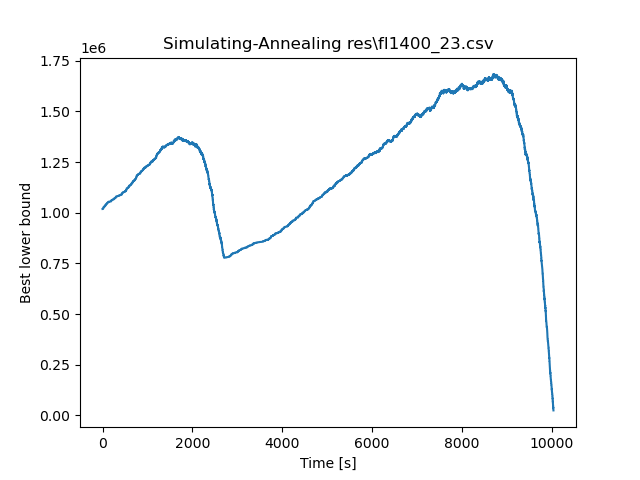
\includegraphics[width=1.0\columnwidth]{../res/fl1400_23.png}
	\caption{Performance profile considering the execution time of 1400 nodes file with timelimit of 10000}
	\label{fig:simultaing_annealing_perform_time}
\end{figure}

\section{Variable Neighborhood Search (VNS)}
This metaheuristic moves from a solution to another iterating two phases:
\begin{enumerate}
	\item optimization
	\item perturbation
\end{enumerate}
The first is done iterating a refining heuristic until a local minimum is found, in this specific case it has been used the \texttt{best\_2\_opt()} algorithm, which is explained in cap \ref{sec:best_2_opt}. After the optimization, a perturbation is applied to leave the local minima, here \texttt{random\_n\_opt()} with $ n=5 $. This algorithm generate a new solution that differ n edges from the first (check at the end of the section for details).
The two phases are iterated until the max number of iterations or time limit occur.\\
Note that the implemented VNS is not optimized to work with multiple thread.\\
In fig \ref{fig:VNS_d2103} is shown the cost of the solution in each \texttt{best\_two\_opt()} step of the VNS. It is interesting to note that most of the time is required for the first descent and after that the first local minimum is found, the best lower bound does not decrease so much.
The calculated tour is plotted in fig \ref{fig:d2103_16}.\\
The performance profiles in fig \ref{fig:Lsubtour_hardfixing_vns_time} and \ref{fig:Lsubtour_hardfixing_vns_lb} show that VNS is faster than the exact algorithm and the returned solution is near the optimum.

\textbf{\texttt{Random\_n\_opt()}.} The n\_opt set of an tour T is the set of tour that have exactly n different edges w.r.t. T. \texttt{Random\_n\_opt()} return a random tour in this set.
\begin{figure}[!h]
	\begin{subfigure}{.5\columnwidth}
		\centering
		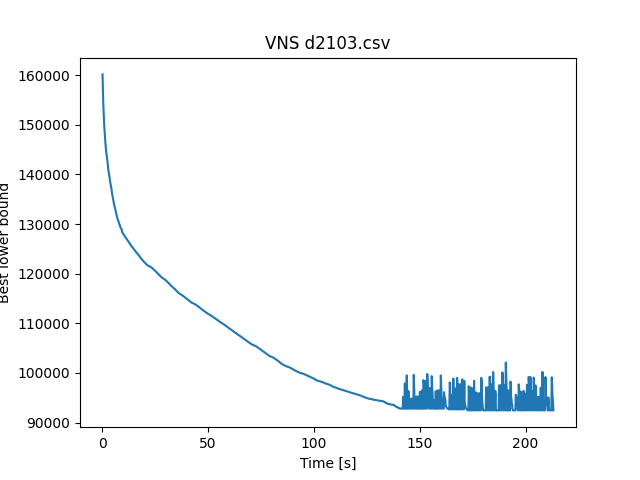
\includegraphics[width=\columnwidth]{../res/d2103.png}
		\caption{The cost of the solution (vs time domain) returned by \texttt{best\_two\_opt()} in each step of the VNS.}
		\label{fig:VNS_d2103}
	\end{subfigure}
	\begin{subfigure}{.5\columnwidth}
		\centering
		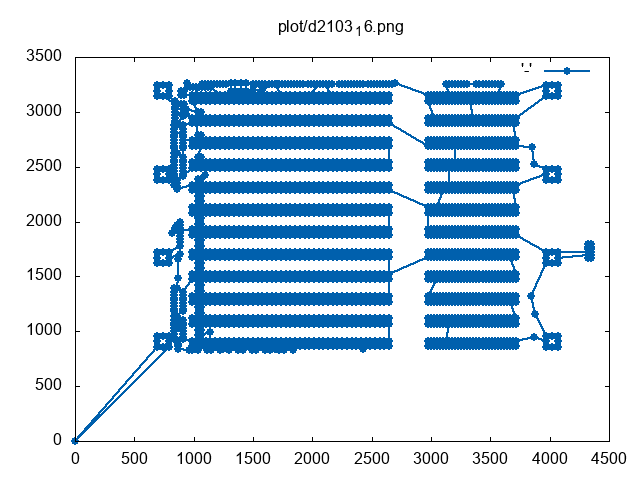
\includegraphics[width=\columnwidth]{../res/d2103_16.png}
		\caption{The graph of the solution returned by VNS.}
		\label{fig:d2103_16}
	\end{subfigure}
	\begin{subfigure}{.5\columnwidth}
		\centering
		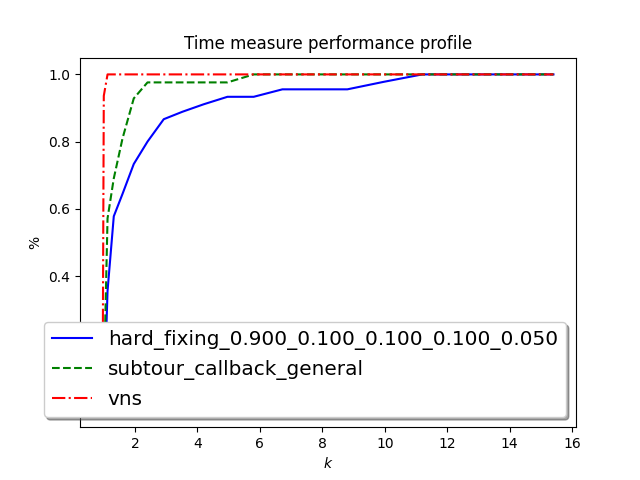
\includegraphics[width=\columnwidth]{../res/Lsubtour_hardfixing_vns_time.png}
		\caption{Performance profile considering the execution time}
		\label{fig:Lsubtour_hardfixing_vns_time}
	\end{subfigure}
	\begin{subfigure}{.5\columnwidth}
		\centering
		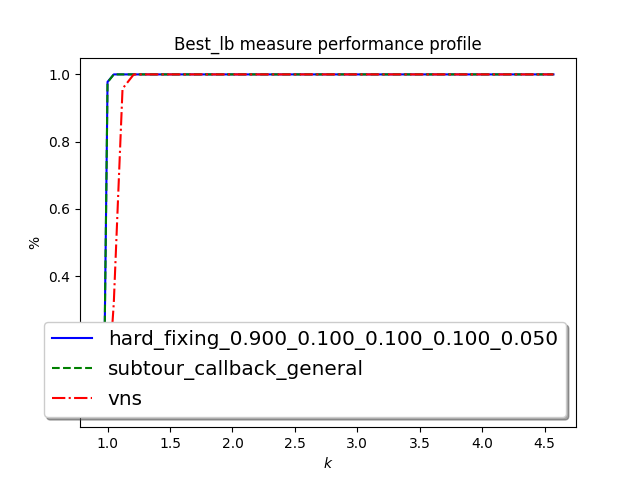
\includegraphics[width=\columnwidth]{../res/Lsubtour_hardfixing_vns_lb.png}
		\caption{Performance profile considering the lower bound.}
		\label{fig:Lsubtour_hardfixing_vns_lb}
	\end{subfigure}
\end{figure}

\section{Genetic Algorithm}
The genetic algorithm (GA) is the last meta-heuristic technique proposed. Its behaviour derives from an evolutionary biology metaphor. A population of individuals (solutions) is randomly created. The individual solutions represent one tour each. These solution are then exposed to simulated evolution.
For a complete explanation of the simple genetic algorithm, see \cite{phdthesis}.\\
A particular genetic algorithm has been implemented in this paper: it is based almost exclusively on the "Powerful Genetic Algorithm Using Edge Assembly Crossover" created by Yuichi Nagata and Shigenobu Kobayashi \cite{Nagata2013, Honda2013}, except for a subsection that has been completely designed by us.\\ A description of the algorithm will be presented and some paragraphs, which are contained in their paper \cite{Nagata2013}, will be reported here thanks to their clear description. In addition, the differences from his algorithm and our implementation choices will be explained.\\
The search process of the GA consists of two stages: \\
\begin{itemize}
\item GA-EAX/Stage I: a localized version of Edge Assembly Crossover (EAX) as the crossover operator from the start of the search until no improvement in the best solution is found over a period of generations or because of timelimit.
\item  GA-EAX/Stage II: after that, switch to a global version of EAX and use it until the end of the search. Stage II is also terminated by the same condition of previous one.
\end{itemize}
For this project only Stage I was developed but the global version does not add any difficulties in the code.

Algorithm \ref{alg:gagen} describes in a compact way the various steps of the entire search.\\

\begin{algorithm}
\caption{GA General}\label{alg:gagen}
\begin{algorithmic}[1]
\Procedure{Procedure GA()}{}
\State $\textit{\{x\textsubscript{$1$},...,x\textsubscript{N\textsubscript{pop}}\}} := \textit{INIT\_POPULATION()}$
\While{\textit{termination condition is satisfied}}
	\State $\textit{r($\cdot$)} := \textit{SHUFFLE\_INDIVIDUALS() $\equiv$ a random permutation of $1$,...,N\textsubscript{pop} } $
	\For{\texttt{$i := 1$ to N\textsubscript{pop}}}
		\State $p_A := \textit{x\textsubscript{r($i$)}} , \textit{p\textsubscript{B}} := \textit{x\textsubscript{r($i+1$)}} $
		\State $\textit{\{y\textsubscript{$1$},...,y\textsubscript{N\textsubscript{kids}}\}} := \textit{EAX\_SINGLE(p\textsubscript{A}, p\textsubscript{B})}$
		\State $\textit{x\textsubscript{r($i$)}} := \textit{SURVIVAL\_SELECTION(y\textsubscript{$1$},...,y\textsubscript{N\textsubscript{kids}}, p\textsubscript{A})} $
	\EndFor
	\State $\textit{best\_individual} := \textit{best individual of actual population}$
\EndWhile
\State \textbf{return} $best\_individual$
\EndProcedure
\end{algorithmic}
\end{algorithm}

\subsection{EAX\_SINGLE}
The recombination operator EAX uses the edges from the two parents to construct disjoint subtours.
Then, using a more general version of the Patching Algorithm \ref{section:patching}, the subtours are connected in a greedy fashion to produce the offspring tour. Thus, the EAX operator considers local information which is exploited in determining which edges to use to connect subtours.\\
Another important trait of the EAX operator is that it will introduce new edges into the offspring when connecting subtours. Edges not in the parents, or perhaps not even in the population, are introduced into offspring. 
The argument as to why good new edges must be introduced during recombination is simple. As point out in \cite{Mathias92geneticoperators}, the complete graph of all possible edges for a symmetric TSP has $(N^2-N)/2$ edges, where $N$ is the number of nodes. Each tour samples $N$ of these edges, so a population must be of size at least $(N-1)/2$ in order to sample each edge exactly once. Assume population size is proportional to the number of the nodes. Then each edge occurs twice in expectation in an initial random population. Selection can therefore quickly eliminate edges from the population. Good edges can also be lost if they occur in poor tours. Thus it is important for operators to intelligently introduce new good edges. This feature is part of the construction of EAX and therefore, may contribute to its effectiveness.\\

\begin{figure}[h]
	\centering
	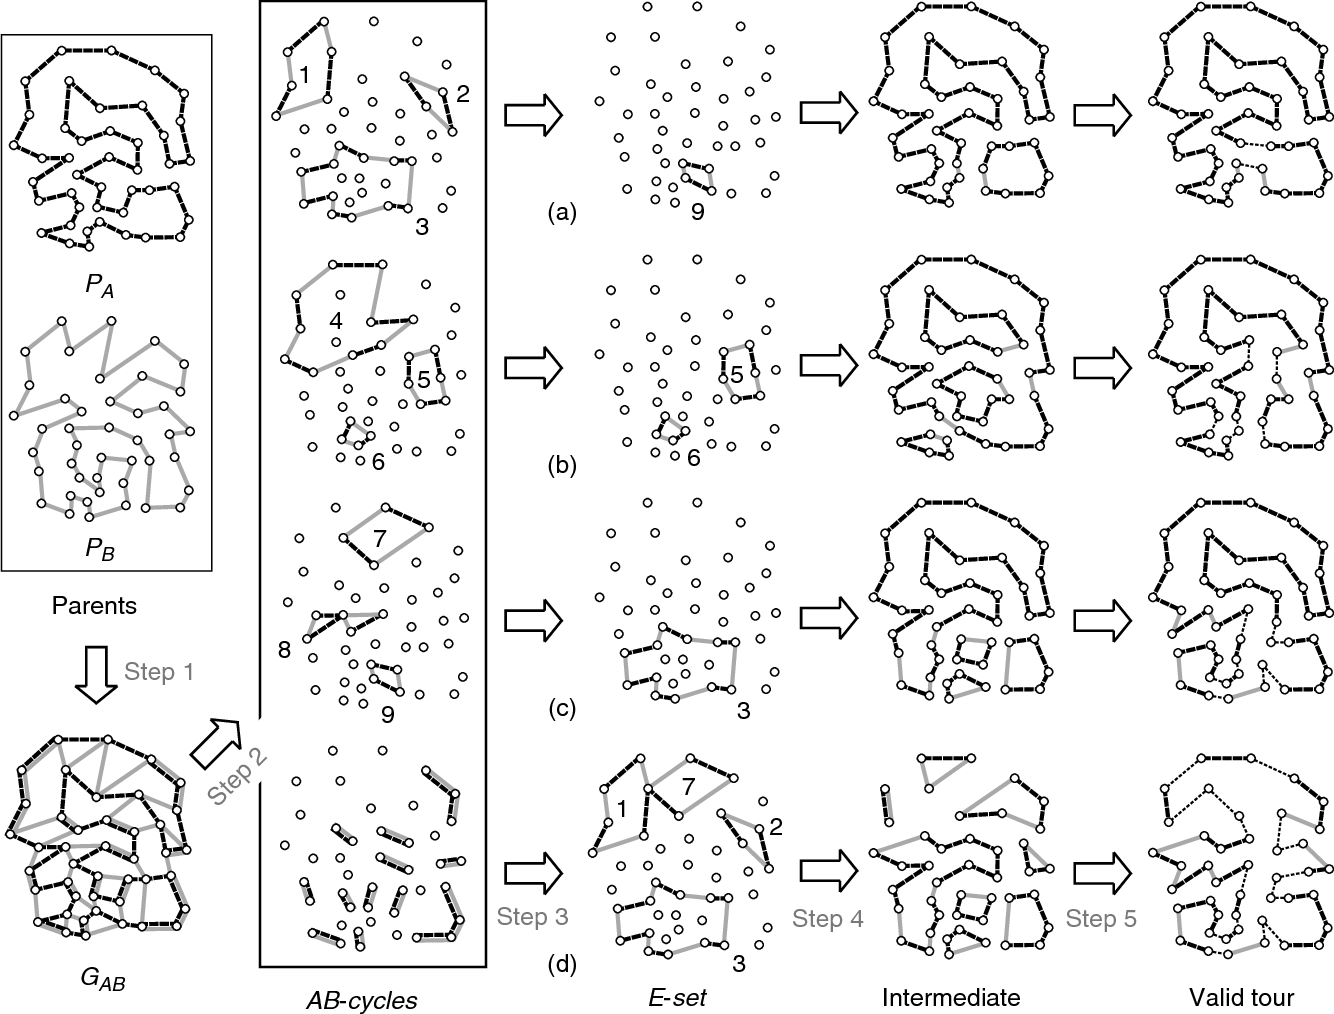
\includegraphics[width=1.0\columnwidth]{img/GA_steps}
	\caption{Example of the EAX\_SINGLE method steps (image taken from \cite{Nagata2013}).}
	\label{fig:GA_steps}
\end{figure}

Focusing on details of the EAX procedure:\\
Once two parents have been selected for crossover, the EAX operator merges these two individuals into a single graph denoted by R (Step 1 of Image \ref{fig:GA_steps}, graph R is named G\textsubscript{AB}). The two parents are denoted by A and B, respectively. Each edge in R is annotated with the parent to which it belongs. R may contain two instances of the same edge, if both parents contain the edge (that is why a more general version of Patching Algorithm is used).\\
R is next divided into a set of disjoint subtours. Let v\textsubscript{i} represent a vertex from R and let (v\textsubscript{i},  v\textsubscript{j}), i $\neq$ j, represent an edge. Suppose (v\textsubscript{i},  v\textsubscript{j}) represents an edge randomly chosen from parent A.\\
Choose one vertex (either v\textsubscript{i} or v\textsubscript{j}) as the origin. If v\textsubscript{i} is the origin, then choose an edge which leads from the second vertex, v\textsubscript{j} , to any other vertex in R. However, this edge must come from parent B. If more than one such edge exists, a random selection is made. The algorithm continues to traverse R, at each step alternately picking edges from parent A and parent B.\\
After each edge is traversed, the algorithm checks to see if adding this new edge to the set of previously selected edges will result in an AB-cycle. An AB-cycle is a even-length sub-cycle of R with edges that alternately come from A and B. An AB-cycle may repeat nodes, but not edges. While there can be two edges between a pair of nodes, they are uniquely identified as an A or B edge, and thus distinct.\\
Once an AB-cycle has been found it is stored and the edges making up that cycle are removed from R. The algorithm repeats this procedure until R contains no more edges, having been completely decomposed into a set of AB-cycles (Step 2 of Image \ref{fig:GA_steps}). \\
The first several edges used in the construction of the AB-cycle may not appear in the final AB-cycle. This occurs when the final edge connects back onto the subgraph at some node x other than the origin node, and the induced subcycle is an AB-cycle. In this case the remaining edges are however removed from R graph but is kept aside in the path being traced, to eventually be used later in forming another cycle. Nagata and Kobayashi choose an edge incident with x from R to begin construction of the next AB-cycle instead in our algorithm we preferred to take an edge incident to any node remaining in the traced path (other technique prefers to select the starting location of a new AB-cycle at random from R).
For the symmetric TSP problem, R is undirected and therefore, the set of AB-cycles is not uniquely determined by the algorithm. Furthermore, a number of "ineffective" AB-cycles may be formed by the algorithm. All AB-cycles that have less than 4 different nodes inside them belong to this group. Any ineffective AB-cycles are found and removed from R and also removed from consideration by the remaining phases of the algorithm.
\\
After construction of the set of AB-cycles, a subset of AB-cycles is chosen to be used in the generation of an intermediate child. This subset is called an E-set (Step 3 of Image \ref{fig:GA_steps}). For selecting AB-cycles for inclusion into the E-set, we choose an our method different from those defined by Nagata and Kobayashi. Given the small size of the problems we tested compared to those of the TSP Art of Nagata, the number of subtours in the E-set is not very large and therefore, instead of sampling by random selection some of them, we scroll through them all and create one intermediate child for each.
\\
Construction of an intermediate child, C, begins with a copy of parent A. Then each edge of each subtour in the E-set is examined, with the following actions taken on C. If the edge from the E-set is a member of parent A, the edge is deleted from C. If the edge is a member of parent B, the edge is added to C. The result is a set of disjoint subtours which comprise the intermediate child (Step 4 of Image \ref{fig:GA_steps}). \\
The last stage of the EAX operator involves transformation of the intermediate child into a single legal tour using a general Patching Algorithm (Step 5 of Image \ref{fig:GA_steps}). The difference between this general algorithm and the one presented in \ref{section:patching} is in the possibility of having double edges, after performing Step 4. This implies that one of the subtours can only be made up of two nodes and two same edges, one of parent A and one of B. Similar situation with three nodes and six edges (three doubles). In previous problems this situation never happened and therefore we generalized the Patching algorithm to include this variant.\\ 
The pseudocode of the EAX\_SINGLE method is identical to that explained in Algorithm 1 of Paper \cite{Honda2013}.

\subsection{Evaluate AB-Cycles}
This method was completely designed by us from scratch. It refers to how to find a cycle that respects the conditions of the EAX\_SINGLE procedure inside the nodes and edges traced so far by the current AB-Cycle. An explanation of this procedure is not given in the papers \cite{Nagata2013, Honda2013} and it is not even that simple. We initially thought of using a greedy graph search algorithm, such as Depth First Traversal (DFT) or Breadth First Search (BFS), but these algorithms do not include the presence of double edges between two nodes and are based on visiting the nodes and not edges and also once found any cycle they stop and do not provide the possibility to continue the search if the cycle does not meet certain conditions. So we have developed an ad hoc algorithm for this type of search that transforms the graph into a tree considering double edges and the possibility to continue the search if a cycle is found that does not respect the conditions required by the EAX\_SINGLE. This algorithm has a recursive structure and uses linked lists that allow a dynamic allocation to save all the necessary information, it was also built trying to free up memory as much as possible in order to avoid overflow as the generations increase. Furthermore, the possibility of finding all the cycles within the graph and not only one is managed, but, as required by the EAX, when an acceptable solution is found, the search ends.

\subsection{SURVIVAL\_SELECTION}
For the survival selection method, some parameters are defined: 

\begin{itemize}
\item N\textsubscript{pop}
\item N\textsubscript{kids}
\item Edge Frequency Table F($e$)
\end{itemize}
N\textsubscript{pop} and N\textsubscript{kids} be the population size and the number of offspring solutions generated from a single pair of parents, p\textsubscript{A} and p\textsubscript{B}, respectively, with the chosen values of 300 and 30, as in the default configuration of GA-EAX/Stage I \cite{Nagata2013}. N\textsubscript{kids} represents an upper bound to the number of offspring solutions but fewer of them could be generated. \\
The edge frequency table F($e$) is a table that records the frequencies of each edge $e \in E$ included in the population, where $E$ is the edge set of the complete graph of a given TSP instance. The values of F($e$) are initialized and are used in the evaluation function for selecting offspring solutions. This evaluation function is based on the edge entropy measure computed from F($e$) and is used for maintaining the population diversity in a positive manner. \\
To keep the table updated: let $y\ssymbol{1}$ be the selected individual among the generated offsprings, which replaces the population member chosen as parent p\textsubscript{A}. The values of F($e$) are updated as follows: 

\begin{equation}\begin{array}{ll}
F(e) \leftarrow F(e)-1 & \forall e \in E\textsubscript{remove} \\
F(e) \leftarrow F(e)+1 & \forall e \in E\textsubscript{add}
\end{array}\end{equation}

where E\textsubscript{remove} is a set of the edges that are included in p\textsubscript{A} but not included in $y\ssymbol{1}$, E\textsubscript{add} is a set of the edges that are included in $y\ssymbol{1}$ but not included in p\textsubscript{A}. \\

The offspring $y\ssymbol{1}$ is selected, taking account of the balance between the amount of the improvement and loss of the population diversity. Let L be the average tour length of the population and H the edge entropy of the population defined as follows:

\begin{equation}
H=-\sum_{e \in E} F(e) / N_{\mathrm{pop}}\left(\log \left(F(e) / N_{\mathrm{pop}}\right)\right)
\end{equation}

$\Delta$L(y) and $\Delta$H(y) denote the differences in L and H, respectively, when x\textsubscript{i}(p\textsubscript{A}) is replaced with $y\ssymbol{1}$. The offspring $y\ssymbol{1}$ is selected so that the following evaluation function is maximized.

\begin{equation}\text { Eval\textsubscript{Ent}}(y):=\left\{\begin{array}{ll}
\frac{\Delta L(y)}{\Delta H(y)} & (\Delta L<0, \Delta H<0) \\
-\frac{\Delta L(y)}{\epsilon} & (\Delta L<0, \Delta H \geq 0) \\
-\Delta L(y), & (\Delta L \geq 0)
\end{array}\right.\end{equation}

where $y$ is an offspring solution and $\epsilon$ is a sufficiently small positive number (our chosen value $0.1$).\\

\subsection{Test}


	\chapter{Constructive Heuristics}

\section{Greedy}
\section{Greedy Randomize Adaptive Search Path (GRASP)}
GRASP metaheuristic, as the name anticipate, is a Greedy constructive heuristic with some randomization. Indeed, for the TSP problem, instead of bring the closer isolated node as next, it's chose a random node between the $ G $ closest isolated nodes, where $ G = 3 $ in the tested implementation.
The idea is that in TSP it's not always the closer to be the next node on the optimum tour. Moreover, in other metaheuristics that start from a solution and optimize it, a percentage of randomness is appreciated.

In figure \ref{fig:att48_diff} can be compared of the optimum tour, the best Greedy and 4 different instances of GRASP. It's nice to see that the best Greedy (fig \ref{fig:att48_GREEDY}) is pretty close to the optimal solution and also some instance of GRASP like \ref{fig:att48_GRASP2} and \ref{fig:att48_GRASP4}

\begin{figure}[h]
	\begin{subfigure}{.5\textwidth}
		\centering
		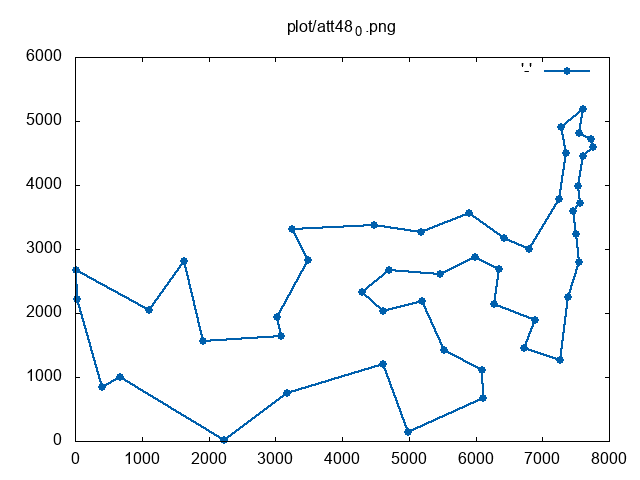
\includegraphics[width=\columnwidth]{../res/att48_0.png}
		\caption{Optimal subtour (cost $ = 10628 $, exec time = $ 0.76 $ s)}
		\label{fig:att48_best}
	\end{subfigure}
	\begin{subfigure}{.5\textwidth}
		\centering
		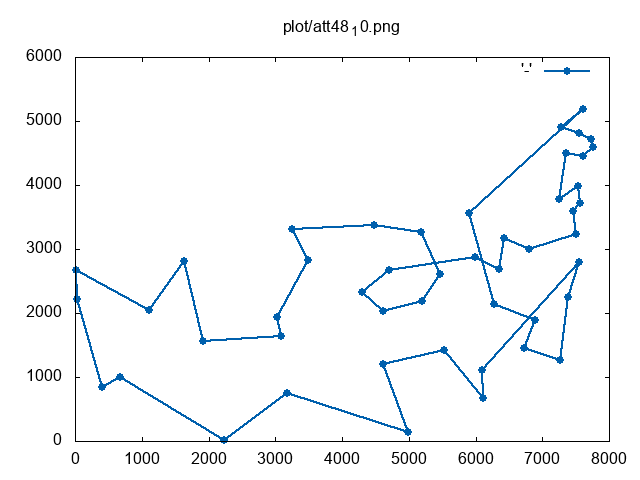
\includegraphics[width=\columnwidth]{../res/att48_10.png}
		\caption{Best Greedy (cost $ = 12012 $, exec time = $ 10^{-6} $s)}
		\label{fig:att48_GREEDY}
	\end{subfigure}
	\begin{subfigure}{.5\textwidth}
	\centering
	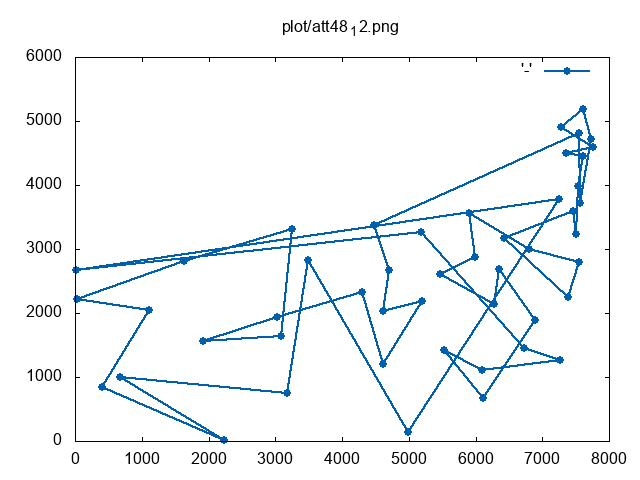
\includegraphics[width=\columnwidth]{../res/att48_12_1.png}
	\caption{GRASP (cost = 21824, exec time = $ 10^{-6} $s)}
	\label{fig:att48_GRASP1}
	\end{subfigure}
	\begin{subfigure}{.5\textwidth}
	\centering
	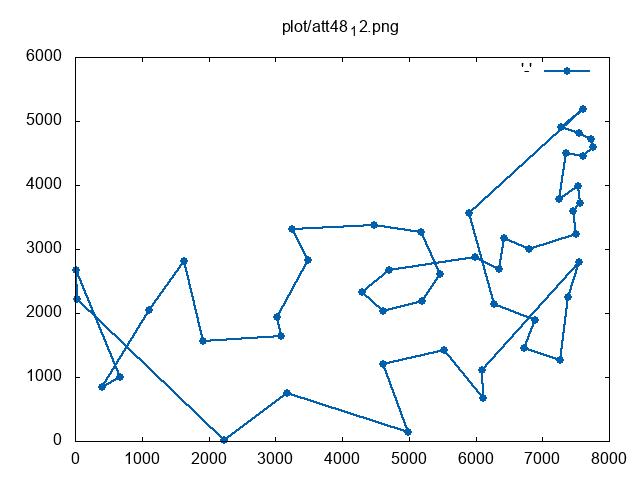
\includegraphics[width=\columnwidth]{../res/att48_12_2.png}
	\caption{GRASP (cost = 12576, exec time = $ 10^{-6} $s)}
	\label{fig:att48_GRASP2}
	\end{subfigure}
	\begin{subfigure}{.5\textwidth}
	\centering
	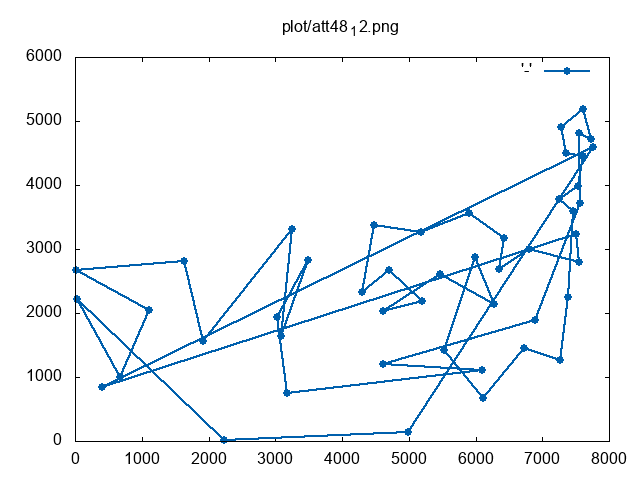
\includegraphics[width=\columnwidth]{../res/att48_12_3.png}
	\caption{GRASP (cost = 22179, exec time = $ 10^{-6} $s)}
	\label{fig:att48_GRASP3}
	\end{subfigure}
	\begin{subfigure}{.5\textwidth}
	\centering
	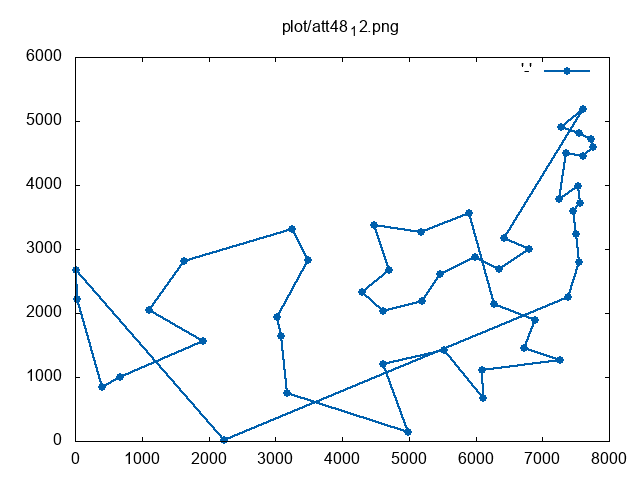
\includegraphics[width=\columnwidth]{../res/att48_12_4.png}
	\caption{GRASP (cost = 13198, exec time = $ 10^{-6} $s)}
	\label{fig:att48_GRASP4}
	\end{subfigure}
	\caption{Differences of Greedy and GRASP tour for att48.tsp instace.}
	\label{fig:att48_diff}
\end{figure}

\section{Insertion Heuristic}

	\chapter{Refining Heuristics}
In this chapter are discussed the heuristic that starting from an initial solution of the TSP, return a better solution in term of cost. This kind of heuristic will be called Refining Heuristics because of the solution cost improvement. 

\section{2-opt} \label{sec:best_2_opt}

This heuristic is a simple and effective local search algorithm for TSP problem.\\
A pseudo-code is proposed in alg. \ref{alg:2opt} to describe how it works. The input parameter $ T $ is an ordered list of edges that define a tour and each edge is represented with an ordered pair of nodes. The \texttt{swap\_edges} method remove the two input edges from the tour $ T $ and add the new edges as show in fig. \ref{fig:2_opt_graph}.

\begin{algorithm}
	\caption{}\label{alg:2opt}
	\begin{algorithmic}[1]
	\Procedure{Procedure 2\_opt}{T}
		\State{\textit{// Variable initialization}}
		\State{$ (n_1, n_2), (m_1, m_2) = T[1], T[3] $}
		\State{$ (n_1^*, n_2^*), (m_1^*, m_2^*) = (n_1, n_2), (m_1, m_2) $}
		\State{$ \delta_{cost}^* = c_{n_1m_1} + c_{n_2m_2} - c_{n_1n_2} - c_{m_1m_2}  $}
		\For{$ (n_1,n_2) \in T $}
			\For{$ (m_1,m_2) \in T $ } \textit{ // For each pair of edge in the tour}
				\If{$ n_1 == m_1 \lor n_1 == m_2 \lor n_2 == m_1 \lor n_2 == m_2 $}
					\State{\textbf{continue}}
				\EndIf
				\State{$ \delta_{cost} = c_{n_1m_1} + c_{n_2m_2} - c_{n_1n_2} - c_{m_1m_2} $}
				\If{$ \delta_{cost} < \delta_{cost}^* $} \textit{ // Find 2-opt candidates}
					\State{$ \delta_{cost}^* = \delta_{cost} $}
					\State{$ (n_1^*, n_2^*), (m_1^*, m_2^*) = (n_1, n_2), (m_1, m_2) $}
				\EndIf
			\EndFor
		\EndFor
		\State{\texttt{swap\_edges($ T, (n_1^*, n_2^*), (m_1^*, m_2^*) $)}}
	\EndProcedure
	\end{algorithmic}
\end{algorithm}

In the example in fig. \ref{fig:2_opt_graph} the pair that has the best improvement is $ (1,4) $ and $ (5,2) $. Note that although $ (5,2) = (2,5) $ for the model, to be coherent with $ \delta_{cost} $ annotation, an orientation of the tour must be choose, and each edge must be represented with consequent ordered node pair: if $ (1,4) $ is the first considered edge, it impose the orientation of the tour.

\begin{figure}[h]
	\centering
	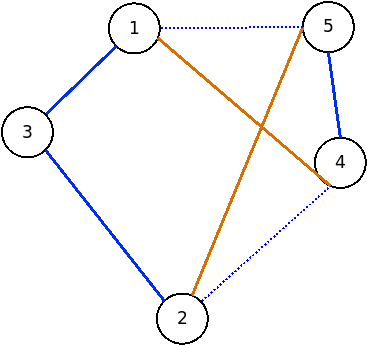
\includegraphics[width=.3\columnwidth]{img/2_opt_graph.png}
	\caption{Example graph to explain \texttt{2\_opt} method. The input graph is that with continuous edges. \texttt{2\_opt} would remove $ (1,4) $ and $ (2,5) $ from the tour and replace them with $ (1,5) $ and $  (2,4) $}
	\label{fig:2_opt_graph}
\end{figure}
As can be seen in fig. \ref{fig:lb_time_grasp_best_two_opt_d2103} multiple execution of \texttt{2\_opt} can improve more than 50\% the cost of the solution before to find a local minimum. This method in the report is called \texttt{best\_two\_opt}.
\begin{figure}[!h]
\centering
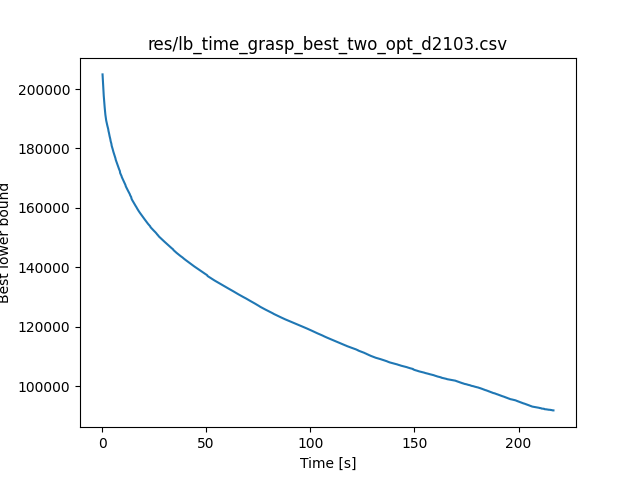
\includegraphics[width=.6\columnwidth]{../res/lb_time_grasp_best_two_opt_d2103.png}
\caption{Solution cost profile of \texttt{best\_two\_opt}. \texttt{GRASP} solution is used as warm start.}
\label{fig:lb_time_grasp_best_two_opt_d2103}
\end{figure}

It is interesting to see the solution cost profile of \texttt{best\_two\_opt} (fig. \ref{fig:a280_25}) applied to the best of the Greedy solutions (called \texttt{greedy\_best\_two\_opt}). The improve of the cost solution is considerable even if it stop on a local minimum.  Note that, the best tour is calculated in about $ 8 $s with \texttt{subtour\_callback\_general}, \texttt{Greedy} take about $ 5 $s to find the \texttt{Greedy} tours and \texttt{best\_two\_opt} find a local minimum in $0.07$s. Moreover is important to consider that \texttt{Greedy} method can be easily modify to execute each Greedy tour in parallel and than apply \texttt{best\_two\_opt}.\\
In fig.s \ref{fig:a280_10} and \ref{fig:a280_25} can be compared the \texttt{Greedy}, \texttt{greedy\_best\_two\_opt} and \texttt{subtour\_callback\_general} tours, solutions cost and execution time.\\

\begin{figure}[!h]
	\begin{subfigure}{.5\columnwidth}
		\centering
		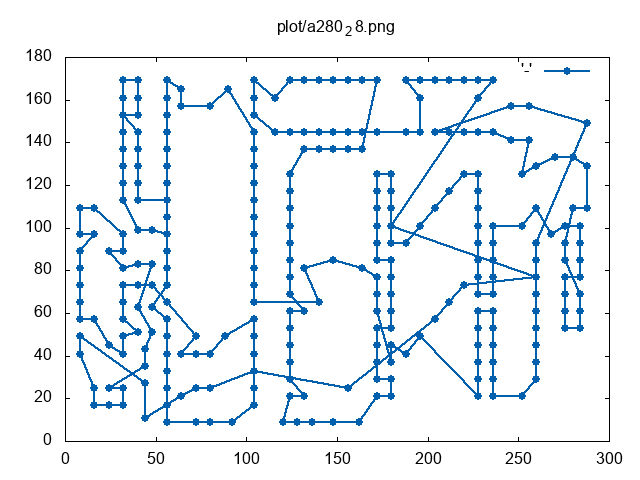
\includegraphics[width=\columnwidth]{../res/a280_28.png}
		\caption{\texttt{n\_greedy\_10}: cost=3078, time=0.45s}
		\label{fig:a280_10}
	\end{subfigure}
	\begin{subfigure}{.5\columnwidth}
		\centering
		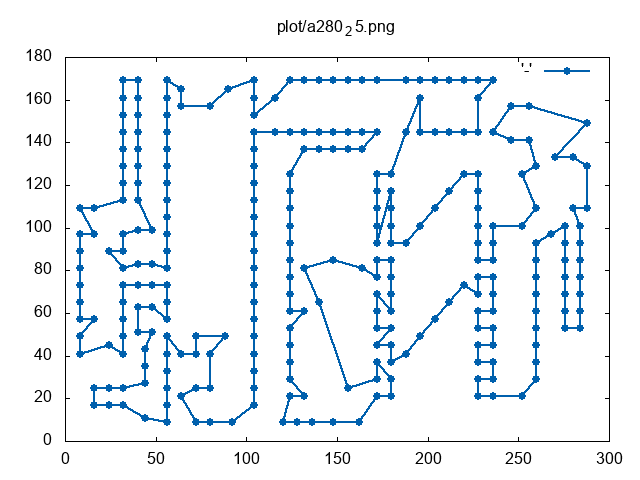
\includegraphics[width=\columnwidth]{../res/a280_25.png}
		\caption{\texttt{n\_greedy\_best\_two\_opt}: cost=2683, time=0.06s}
		\label{fig:a280_25}
	\end{subfigure}
	\begin{subfigure}{.5\columnwidth}
		\centering
		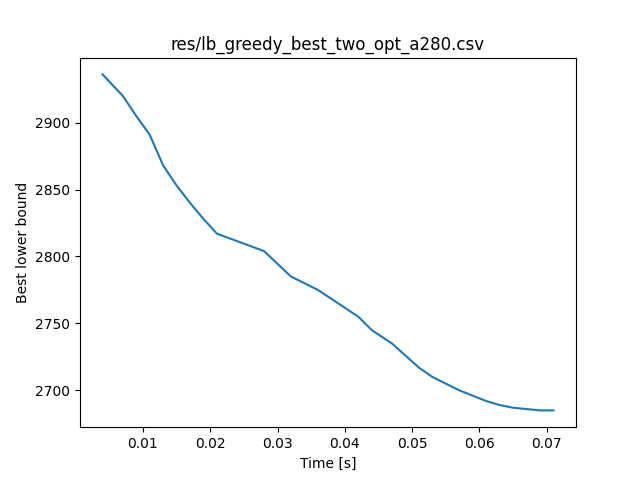
\includegraphics[width=\columnwidth]{../res/lb_greedy_best_two_opt_a280.png}
		\caption{The profile of the solution cost over time of the \texttt{best\_two\_opt} optimization phase.}
		\label{fig:lb_greedy_best_two_opt_a280}
	\end{subfigure}
	\begin{subfigure}{.5\columnwidth}
		\centering
		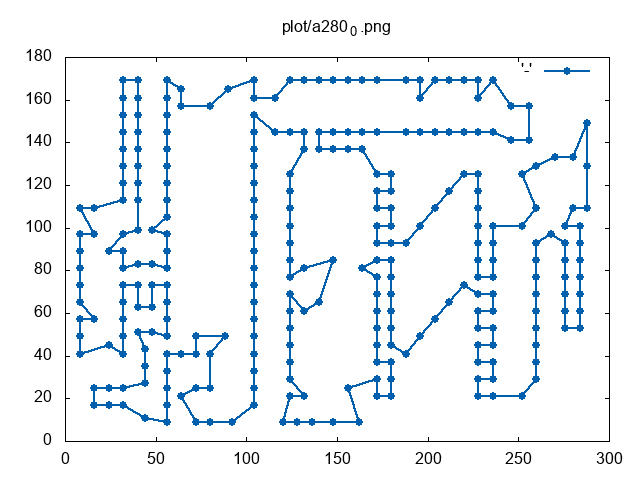
\includegraphics[width=\columnwidth]{../res/a280_0.png}
		\caption{\texttt{subtour\_callback\_general}: cost=2579, time=8s}
		\label{fig:a280_0}
	\end{subfigure}
\end{figure}


\begin{figure}[!h]
	\centering
	\begin{subfigure}{.7\textwidth}
		\centering
		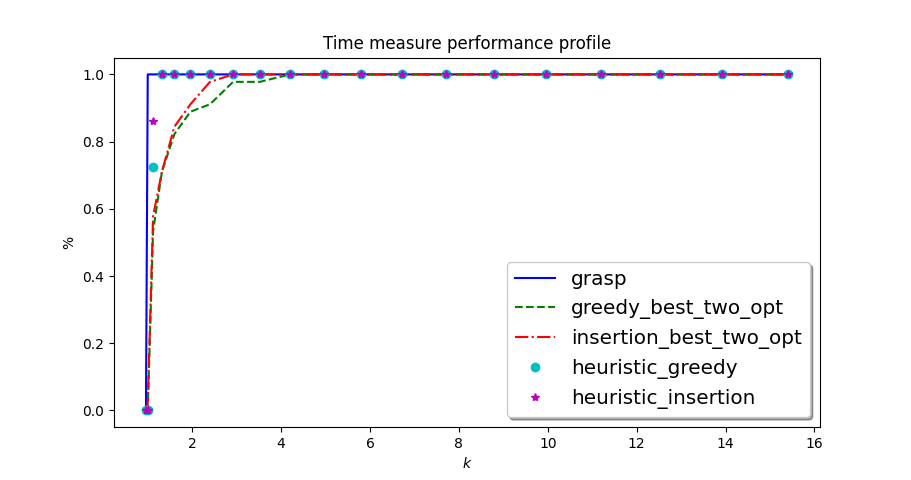
\includegraphics[width=\columnwidth]{../res/Lconstructives_refining_LA_time.png}
		\caption{Performance profile in time domain.}
		\label{fig:Lconstructives_refining_time}
	\end{subfigure}
	\begin{subfigure}{.7\textwidth}
		\centering
		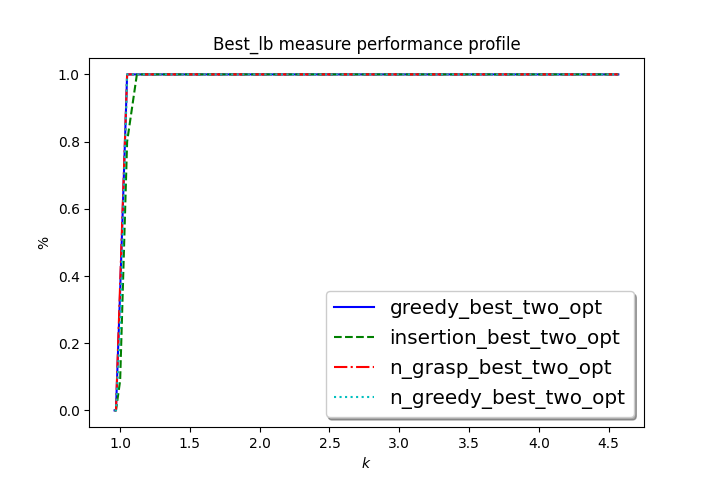
\includegraphics[width=\columnwidth]{../res/Lconstructives_refining_LA_lb.png}
		\caption{Performance profile in solution cost domain.}
		\label{fig:Lconstructives_refining_lb}
	\end{subfigure}
\caption{Performance profile of refining heuristic}
\label{fig:pp_Lconstructives_refining}
\end{figure}

The performance profile in fig. \ref{fig:pp_Lgreedy_refining} compare greedy algorithms with them \texttt{best\_two\_opt} optimization. It is clear that most of the execution time is required for the constructive heuristic, however the difference in term of cost optimization is done by the \texttt{best\_two\_opt}. In fig. \ref{fig:Lgreedy_refining_LA_lb} \texttt{n\_greedy\_best\_two\_opt} gain the solution of \texttt{greedy\_best\_two\_opt}, proving that it is not necessary to find the best tour created from the greedy, but is enough to compute ten random tour and than apply \texttt{best\_two\_opt} to find similar solution cost.

\begin{figure}
	\centering
	\begin{subfigure}{.8\textwidth}
		\centering
		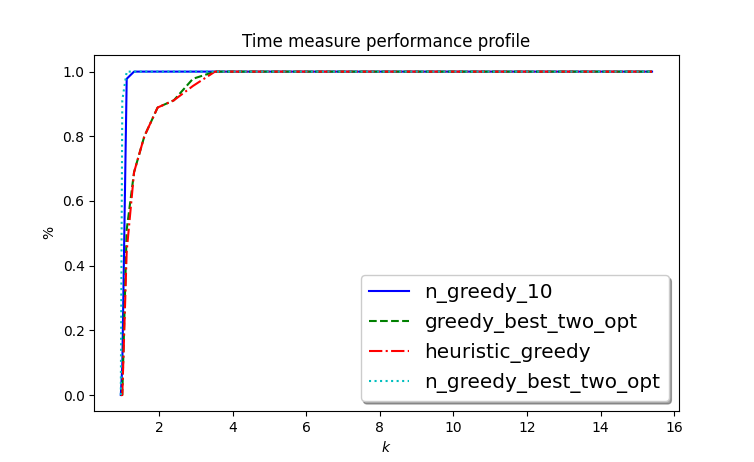
\includegraphics[width=\columnwidth]{../res/Lgreedy_refining_LA_time.png}
		\caption{Performance profile in solution cost domain.}
		\label{fig:Lgreedy_refining_LA_time}
	\end{subfigure}
	\begin{subfigure}{.8\textwidth}
		\centering
		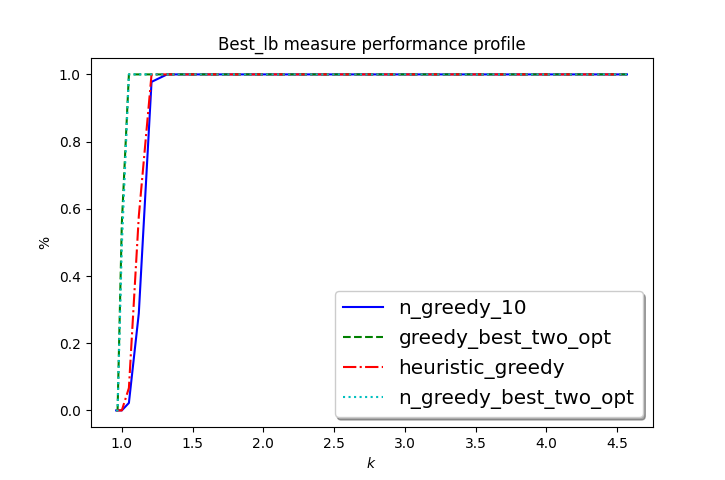
\includegraphics[width=\columnwidth]{../res/Lgreedy_refining_LA_lb.png}
		\caption{Performance profile in solution cost domain.}
		\label{fig:Lgreedy_refining_LA_lb}
	\end{subfigure}
	\caption{Comparison of constructive vs refining heuristics of greedy methods.}
	\label{fig:pp_Lgreedy_refining}
\end{figure}


The effectiveness of the refining heuristic depend from the warm start solution. In fig. \ref{fig:Lgrasp_insertion_refining_LA_lb} it is show that even if \texttt{heuristic\_insertion} generate shorter tour than \texttt{n\_grasp}, \texttt{n\_grasp\_best\_two\_opt} is better than \texttt{insertion\_best\_two\_opt}.

\begin{figure}
\centering
\begin{subfigure}{.7\textwidth}
	\centering
	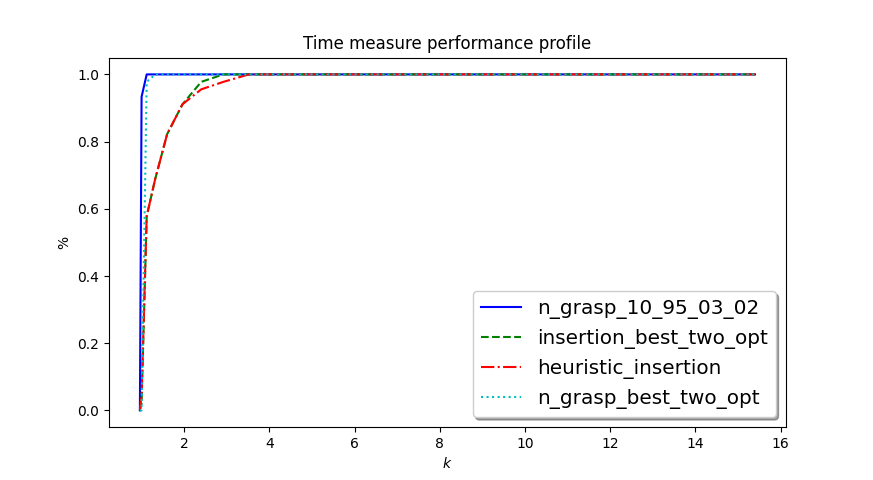
\includegraphics[width=\columnwidth]{../res/Lgrasp_insertion_refining_LA_time.png}
	\caption{Performance profile in solution cost domain.}
	\label{fig:Lgrasp_insertion_refining_LA_time}
\end{subfigure}
\begin{subfigure}{.7\textwidth}
	\centering
	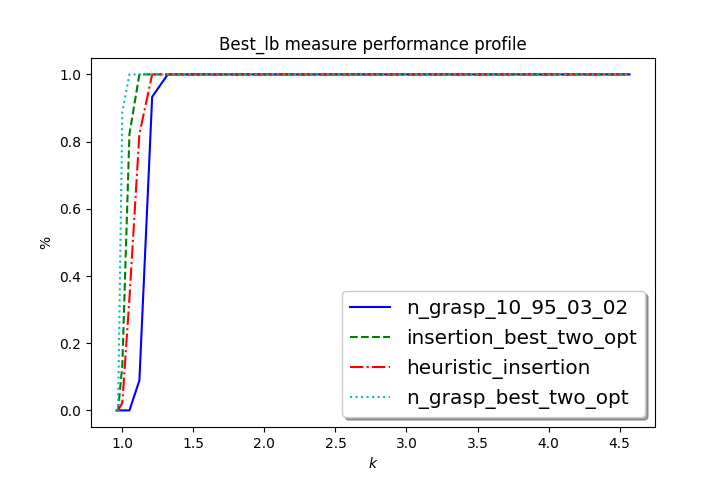
\includegraphics[width=\columnwidth]{../res/Lgrasp_insertion_refining_LA_lb.png}
	\caption{Performance profile in solution cost domain.}
	\label{fig:Lgrasp_insertion_refining_LA_lb}
\end{subfigure}
\caption{Comparison of constructive vs refining heuristics of grasp and insertion methods.}
\label{fig:pp_Lgrasp_insertion_refining}
\end{figure}

In conclusion, \texttt{best\_two\_opt} is a really useful refining heuristic for its time efficiency and cost effectiveness, however its effectiveness depend from how many cross edges has the warm start solution.

	\chapter{Repair}
\section{Patching} \label{section:patching}
The Patching heuristic is a way to merge together multiple tours and obtain a single one.
The algorithm proposed is an iteration of a \texttt{single\_patch()} method which merge only one pair of tours. Note that an isolated node is the tour with minimum length therefore \texttt{patching()} can also resolve a TSP problem. \\
The proposed algorithm work through the 6 step presented in fig \ref{fig:single_patch}.
\begin{figure}[!h]
	\begin{subfigure}{.26\columnwidth}
		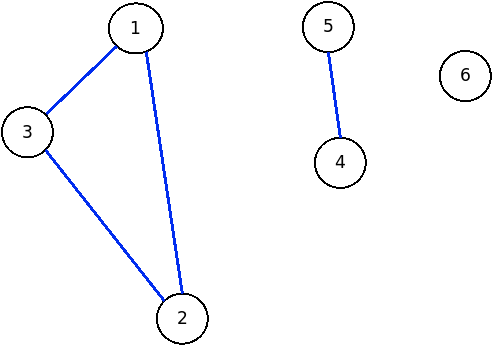
\includegraphics[width=\columnwidth]{img/patching1.png}
		\caption{The single patch input instance.}
		\label{fig:patching1}
	\end{subfigure}
\hfill%
	\begin{subfigure}{.26\columnwidth}
		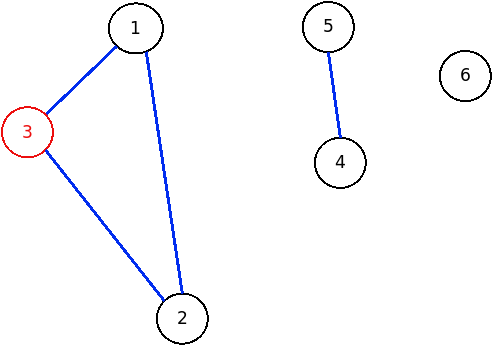
\includegraphics[width=\columnwidth]{img/patching2.png}
		\caption{Node $ 3 $ is chosen randomly from a set of subtours.}
		\label{fig:patching2}
	\end{subfigure}
\hfill%
	\begin{subfigure}{.26\columnwidth}
		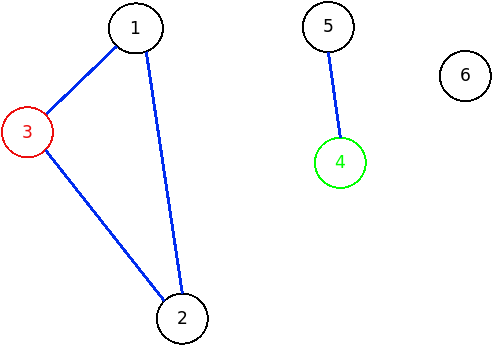
\includegraphics[width=\columnwidth]{img/patching3.png}
		\caption{It is selected the closer node to $ 3 $ which is a different tour (node $ 4 $).}
		\label{fig:patching3}
	\end{subfigure}
	\begin{subfigure}{.26\columnwidth}
		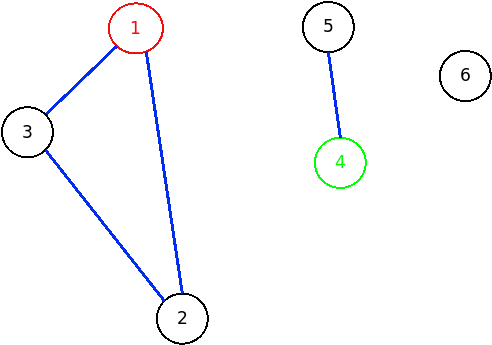
\includegraphics[width=\columnwidth]{img/patching4.png}
		\caption{Iterating throw the first tour nodes, it is selected the node which minimize the next merge cost.}
		\label{fig:patching4}
	\end{subfigure}
\hfill%
	\begin{subfigure}{.26\columnwidth}
		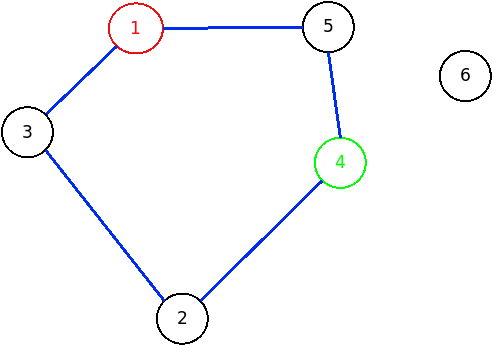
\includegraphics[width=\columnwidth]{img/patching5.png}
		\caption{Merge operation.}
		\label{fig:patching5}
	\end{subfigure}
\hfill%
	\begin{subfigure}{.26\columnwidth}
		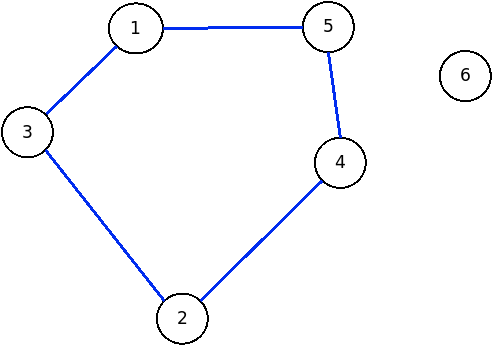
\includegraphics[width=\columnwidth]{img/patching6.png}
		\caption{The final result.}
		\label{fig:patching6}
	\end{subfigure}
\caption{Single patch move algorithm}
\label{fig:single_patch}
\end{figure}\\
A \texttt{succ} structure is use to represent the input tours, which for each  $ i = 1, .., n = |V|$ is defined as: 
\begin{equation}
\texttt{succ[i] = } \begin{cases}
 \text{"\texttt{i} successor"} & \text{if \texttt{i} is in a tour,}\\
 \text{\texttt{-1}} & \text{otherwise.}
\end{cases}
\end{equation} \\
In the \texttt{succ} structure, each edge could be considered as oriented: if \texttt{succ[i] = j} than \texttt{i} $\rightarrow$ \texttt{j} is the considered edge orientation. \\
The merge phase is the core of the method. To avoid a large number of intersection between edges, which is a sign of non optimal solution, all the tour are initialize in clockwise orientation and the merge phase keep the property in the output tour. An example of merge is done in fig \ref{fig:patching_merge}.
\begin{figure}[!h]
	\begin{subfigure}{.26\columnwidth}
		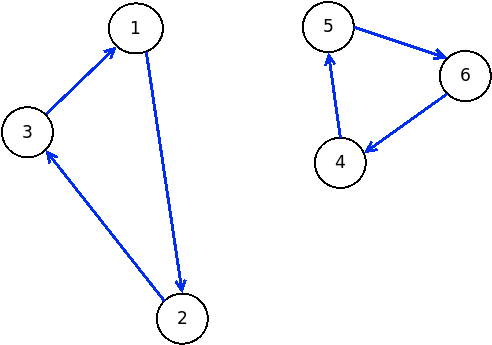
\includegraphics[width=\columnwidth]{img/patching_merge1.png}
		\caption{}
		\label{fig:patching_merge1}
	\end{subfigure}
	\hfill%
	\begin{subfigure}{.26\columnwidth}
		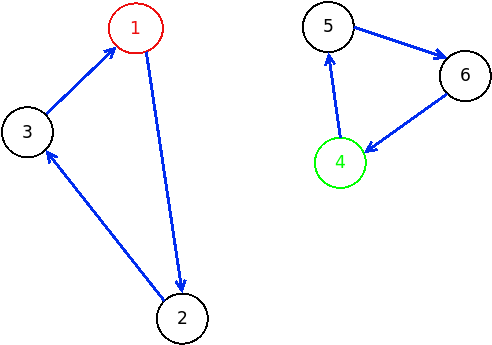
\includegraphics[width=\columnwidth]{img/patching_merge2.png}
		\caption{}
		\label{fig:patching_merge2}
	\end{subfigure}
	\hfill%
	\begin{subfigure}{.26\columnwidth}
		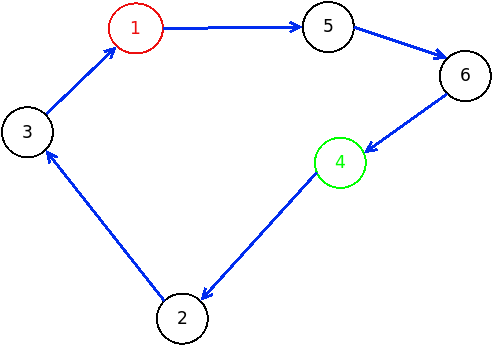
\includegraphics[width=\columnwidth]{img/patching_merge3.png}
		\caption{}
		\label{fig:patching_merge3}
	\end{subfigure}

	\caption{Merge phase in detail.}
	\label{fig:patching_merge}
\end{figure}\\

\begin{table}[h]
	\centering
	\caption{The \texttt{succ} structure for the tour in figure \ref{fig:patching_merge}}
	\begin{tabular}{clcccccc}
		\multirow{2}{*}{\ref{fig:patching_merge1})} 	& \texttt{i:}		& 1 & 2 & 3 & 4 & 5 & 6 \\
														& \texttt{succ[i]:}	& 2 & 3 & 1 & 5 & 6 & 4 \\
														&		   			&   &   &   &   &   &   \\
		\multirow{2}{*}{\ref{fig:patching_merge3})} 	& \texttt{i:}		& 1 & 2 & 3 & 4 & 5 & 6 \\
														& \texttt{succ[i]:}	& 5 & 3 & 1 & 2 & 6 & 4 \\
	\end{tabular}
\end{table}
To keep the clockwise orientation of the tour there is a special consideration have to be done to merge an isolated node with a tour of two nodes. In the final tour the clockwise property is checked if the condition is satisfied:
$ (x_3 - x_1)*(y_2 - y_1) < (y_3 - y_1)*(x_2 - x_1) $,
otherwise the tour is reversed.


\begin{figure}[!h]
	\hfill%
	\begin{subfigure}{.2\columnwidth}
		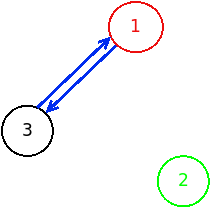
\includegraphics[width=\columnwidth]{img/patching_merge_clockwise1.png}
		\caption{}
		\label{fig:patching_merge_clockwise1}
	\end{subfigure}
\hfill%
	\begin{subfigure}{.46\columnwidth}
		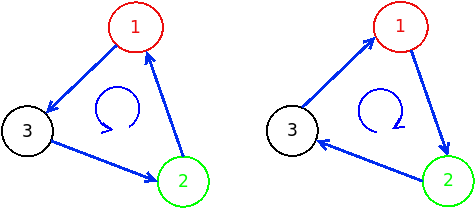
\includegraphics[width=\columnwidth]{img/patching_merge_clockwise2.png}
		\caption{}
		\label{fig:patching_merge_clockwise2}
	\end{subfigure}
\hfill%
	\caption{Special case of merge phase that create a tour with 3 edges.}
	\label{fig:patching_merge_clockwise}
\end{figure}

	\chapter{MIP Heuristics}
Mixed Integer Program Heuristics can be applied in each MIP problem independently from the context. These do not consider the specific formulation of the TSP problem however they could have good applicability. In this report two MIP Heuristics will be discussed and compared with the metaheuristics.

\section{Hard-fixing}
A simple idea to reduce the complexity of the problem is to get an initial solution like an incumbent, fix some active edges and resolve the subproblem with CPLEX. This is exactly the idea behind hard fixing approach.\\
The implementation proposed is applied in sTSP problem, with the optimization of the general callback (\texttt{subtour\_callback\_general}).
The algorithm can be divided in steps:
\begin{enumerate} \label{hard-fix-step}
	\item Calculate an initial solution: in our implementation this is done by CPLEX with \texttt{subtour\_callba \\ ck\_general} and \texttt{CPX\_PARAM\_INTSOLLIM} set to 1. When the first incumbent is available, the optimization terminate and a solution is obtained.
	\item Fix a percentage of edges (fixing rate $ f_r $): edges are fixed using \texttt{CPXchgbds} method that change the upper and lower bound of the decision variables. The fixing percentage is an important parameter: fixing too much edges leads to a fast resolution of the subproblem, however increase the risk of obtaining the same solution and fall in a loop. Fixing too low edges involves slower resolution. In the first iteration $ f_r = 0.9 $.
	\item CPLEX optimization with time limit: After the fixing phase, the problem is optimized with \texttt{CPX\_mipopt} and a short time limit is set (in our implementation $50 $s).
	\item Fixing rate update: after the last phase, if the returned solution is improved better than a fixed gap ($  good\_gap $), it is considered a good solution and the $ f_r $ increases by a constant ($ incr\_f_r $) until a max ($ max\_f_r $), otherwise if the new solution is not increased enough (less than $ optimal\_gap $), then $ f_r $ decreases of a constant ($ decr\_f_r $) until a min ($ min\_f_r $). Note that $ good\_gap $ and $ optimal\_gap $ are expressed as fraction of the current best lower bound.
	\item Check end condition: if the time limit is reached or $ f_r = 0.0 $ and the solution is not improved in the last iteration, then the solution is returned. In the second case, the best solution is found. If no ending condition is satisfied, the algorithm continue with point 3.
\end{enumerate}

\section{Local-Branching}
The Local Branching is a relatively recent algorithm developed by Matteo Fischetti and Andrea Lodi, who wanted to propose an alternative method to Hard Fixing. The Hard Fixing idea, as stated above, fix randomly a percentage of edges and optimize the problem, Local Branching, instead, let the MIP model to fix the percentage of edges automatically and than optimize. \\
Consider $ x^H $ as non optimal tour and $ \chi $ the fraction of edges to fix, Local Branching add
\begin{equation}
 \sum_{ e\in E: x_e^H = 1 } x_e \ge \chi n
\end{equation}
to automatically fix the desired number of edges. \\
In this paper, the structure of the algorithm is very similar to that of Hard Fixing. Initialization is analogous to Point 1 (\ref{hard-fix-step})
In the CPLEX optimization with time limit (Point 3), the time limit is a little higher and is set to 300 according to the choice of the fixing rate update. Thus, the fixing rate is an array consisting of 5 values {3.0, 5.0, 10.0, 15.0, 20.0}. It starts from the first value of 3.0 which is kept until better solutions are found. It is updated to the next value as soon as the algorithm returns a non-improving solution.  \\
This choice is motivated by the idea that keeping a low fixing rate allows you to find a solution in a short time and therefore not reach the time limit, which instead is set with a higher value to allow a longer search when the fixed\_rate increase. \\
If the last value is reached and there is still no improvement solution, then the value is doubled until either a better solution is found or the number of nodes of the problem is reached. In the latter case, the search no longer has any constraint and therefore appears to be the last possible, in fact it is assigned the entire remaining time. \\
The exit conditions evaluate both the time limit and the gap calculated by CPLEX, obtainable through the \texttt{generic\_callback} using \texttt{CPX\_CALLBACKCONTEXT\_GLOBAL\_PROGRESS} as \texttt{Context}. 
For a detailed explanation of the reasons for this algorithm refer to \cite{article}.


\begin{figure}[h]
	\centering
	\begin{subfigure}{\columnwidth}
		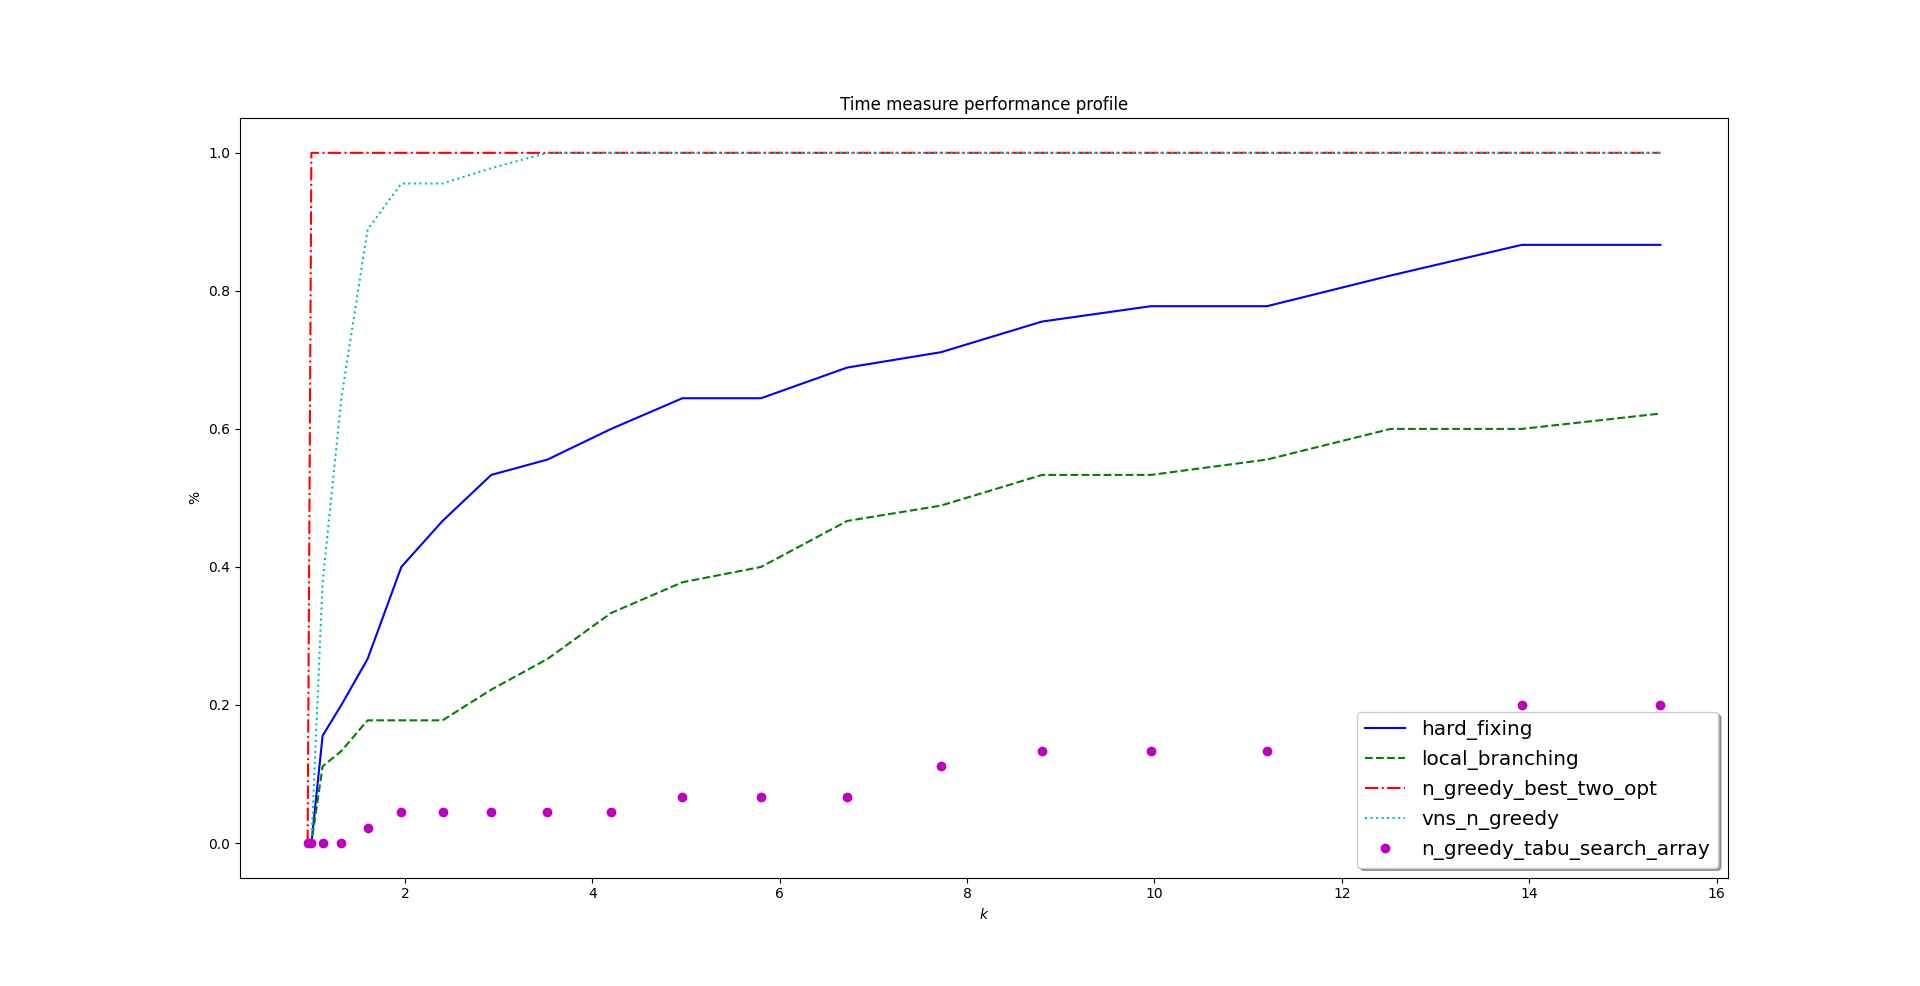
\includegraphics[width=\columnwidth]{../res/Lmip_meta_LA_time.png}
		\caption{}
		\label{fig:Lmip_meta_LA_time}
	\end{subfigure}
	\begin{subfigure}{\columnwidth}
		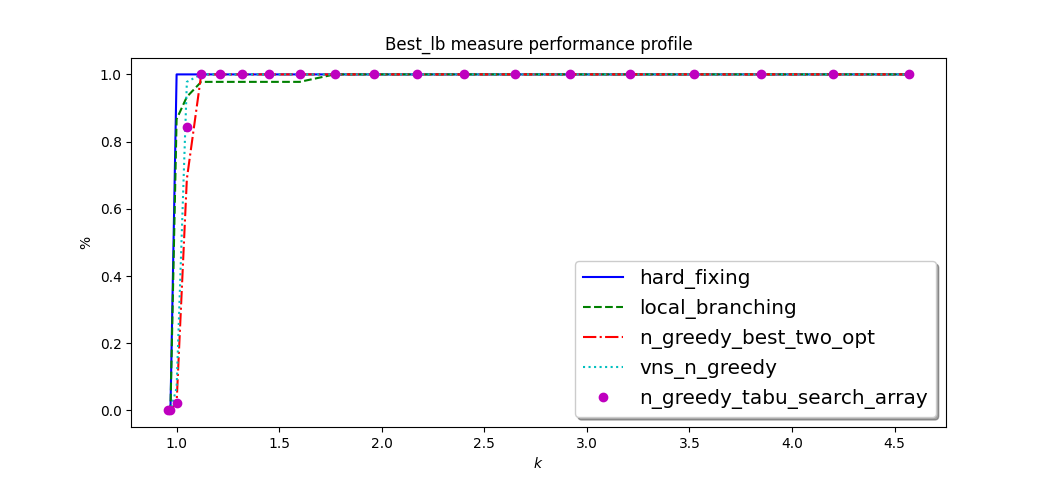
\includegraphics[width=\columnwidth]{../res/Lmip_meta_LA_lb.png}
		\caption{}
		\label{fig:Lmip_meta_LA_lb}
	\end{subfigure}
\caption{Comparison of mip heuristics and meta heuristics. \texttt{n\_greedy\_best\_two\_opt} is the first part of \texttt{vns} therefore it is faster, however the last one introduce a little improvement in the solutions cost. Most of the times \texttt{hard\_fixing} can find the best solution of sTSP indeed it find the shorter tours of the analyzed heuristics. }
\label{fig:Lmip_meta_LA}
\end{figure}

%\section{RINS}
%\section{Feasibility Pump}
%\section{Proximity Search}
%\section{Polishing}

	\chapter{Conclusion}
In conclusion, different MIP exact model have been developed to resolve the TSP problem and \texttt{subtour\_callback\_general} has definitely obtain the best results in term of times. However no exact algorithm can resolve a problem with more than 1000 nodes in less than 600s. This must be considered in particular when the execution time is limited. In this case heuristics can be successfully applied to obtain a good solution (not the best) about 10 times faster. This result are confirmed with the performance profile in fig \ref{fig:pp_Lbest}.\\
For the heuristics, \texttt{best\_two\_opt} obtain really good results in term of execution time and cost optimization, indeed the best heuristic are the constructive ones combined with the iteration of \texttt{best\_two\_opt}.
The constructive \texttt{n\_greedy} achieves the best performances as a heuristic alone but the use of the \texttt{n\_grasp} as a warm start brings a more variability.
\begin{figure}[!h]
	\centering
	\begin{subfigure}{.49\textwidth}
		\centering
		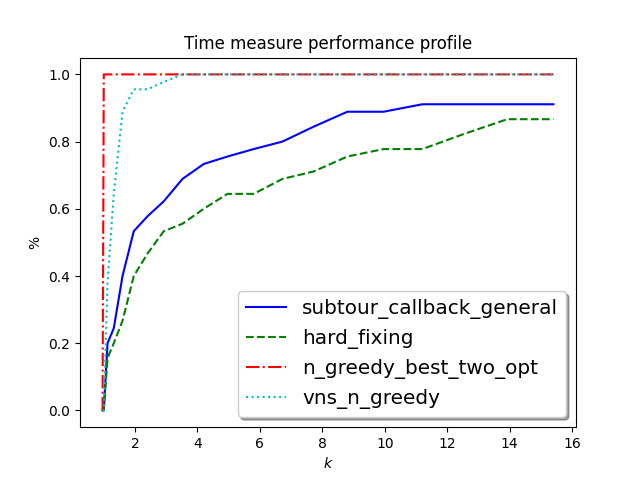
\includegraphics[width=\columnwidth]{../res/Lbest_time.png}
		\caption{Performance profile in time domain.}
		\label{fig:Lbest_time}
	\end{subfigure}
\hfill
	\begin{subfigure}{.49\textwidth}
		\centering
		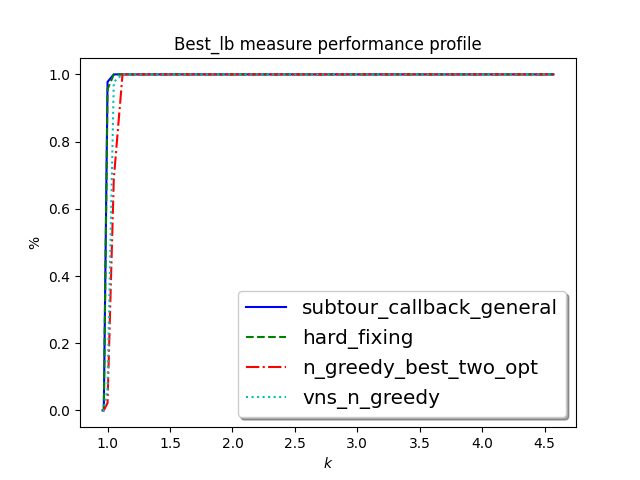
\includegraphics[width=\columnwidth]{../res/Lbest_lb.png}
		\caption{Performance profile in solution cost domain.}
		\label{fig:Lbest_lb}
	\end{subfigure}
	\caption{Performance profile of the best models executed in the union of \textit{data\_light} and \textit{data\_average}.}
	\label{fig:pp_Lbest}
\end{figure}
	\clearpage
	
	\begin{appendices}
		\chapter{Test bed} \label{sec:testset}
		The TSPLIB \cite{TSPLIB} is a library that contain different instances of TSP problem and its best solution found. All the file described in this section are part of the TSPLIB. To test the developed algorithm three different set have been prepared, depending on the number of node ($=|V|$) in the graph: Data Light, Data Average and Data Heavy.\\
		These are all intended as STSP, however the same instance can be considered also for ATSP replacing each edge with two arches with opposite direction. This subdivision is justified by the different execution time of the algorithms: it is more interesting to compare the performance of different algorithms in similar instances.\\
		
		\textbf{Data Light:}
		\begin{multicols}{4}
			\begin{itemize}
				\item att48.tsp
				\item berlin52.tsp
				\item bier127.tsp
				\item burma14.tsp
				\item ch130.tsp
				\item ch150.tsp
				\item eil101.tsp
				\item eil51.tsp
				\item eil76.tsp
				\item gr137.tsp
				\item gr96.tsp
				\item kroA100.tsp
				\item kroA150.tsp
				\item kroB100.tsp
				\item kroB150.tsp
				\item kroC100.tsp
				\item kroD100.tsp
				\item kroE100.tsp
				\item lin105.tsp
				\item pr107.tsp
				\item pr124.tsp
				\item pr136.tsp
				\item pr144.tsp
				\item pr76.tsp
				\item rat99.tsp
				\item rd100.tsp
				\item st70.tsp
				\item ulysses16.tsp
				\item ulysses22.tsp
			\end{itemize}
		\end{multicols}
		
		
		\textbf{Data Average:}
		\begin{multicols}{4}
			\begin{itemize}
				\item a280.tsp
				\item d198.tsp
				\item gil262.tsp
				\item gr202.tsp
				\item gr229.tsp
				\item kroA200.tsp
				\item kroB200.tsp
				\item pr152.tsp
				\item pr226.tsp
				\item pr264.tsp
				\item pr299.tsp
				\item rat195.tsp
				\item rkoA200.tsp
				\item ts225.tsp
				\item tsp225.tsp
				\item u159.tsp
			\end{itemize}
		\end{multicols}
		
		
		\textbf{Data Heavy:}
		\begin{multicols}{4}
			\begin{itemize}
				\item ali535.tsp
				\item att532.tsp
				\item brd14051.tsp
				\item d1291.tsp
				\item d1655.tsp
				\item d18512.tsp
				\item d2103.tsp
				\item d493.tsp
				\item d657.tsp
				\item fl1400.tsp
				\item fl1577.tsp
				\item fl3795.tsp
				\item fl417.tsp
				\item fnl4461.tsp
				\item gr431.tsp
				\item gr666.tsp
				\item nrw1379.tsp
				\item p654.tsp
				\item pcb1173.tsp
				\item pcb3038.tsp
				\item pcb442.tsp
				\item pr1002.tsp
				\item pr2392.tsp
				\item pr439.tsp
				\item rat575.tsp
				\item rat783.tsp
				\item rd400.tsp
				\item rl11849.tsp
				\item rl1304.tsp
				\item rl1323.tsp
				\item rl1889.tsp
				\item rl5915.tsp
				\item rl5934.tsp
				\item u1060.tsp
				\item u1432.tsp
				\item u1817.tsp
				\item u2152.tsp
				\item u2319.tsp
				\item u574.tsp
				\item u724.tsp
				\item usa13509.tsp
				\item vm1084.tsp
				\item vm1748.tsp
			\end{itemize}
		\end{multicols}
		
		\chapter{Performance measure} \label{sec:performance_meausure}
			In this chapter is discussed how the different deveeloped algorithms have been compared between each other.\\
			\textbf{Performance profile.} Exact algorithm (e.g. Subtour, MTZ and FC) guarantee to return the least expensive tour if would run for enough time, therefore a metric of interest is the total execution time needed to find the optimum. 
			Due to practical limitation, a time limit must be imposed. The performance profile compare for each tested instance ($ i $), the ratio ($ r^A(i) = \frac{t_{exec}^A(i)}{t_{exec}^*(i)} $) of the execution time of the algorithm A ($ t_{exec}^A(i) $) divided by the execution time of the faster algorithm ($ t_{exec}^*(i) $), for each $ k = 1, 2, .., K $ calculate the percentage expressed in fraction ($ \% $) of how many instances the algorithm A has $ r^A(i) \le k $ and the resultant function is the performance profile.
			The algorithm with the higher curve is the one who have been for more instances near the best.\\
			A problem of the performance profile is that some instances require fractions of second to be executed and little overhead would significantly influence the performance profile, however the purpose of this report is to measure the instance computability. For example if the faster algorithm run in 0.1s and A in 1s, $ r^A(i_1) = 10 $, which, for the performance profile, would be comparable to a second case where $ t_{exec}^*(i_2) = 100 $s and $ t_{exec}^A(i_2) = 1000 $s. To enhance the weight of the second cases, the calculated ratio is modified as follow: $ r^A(i) = \frac{t_{exec}^A(i)+T_{min}}{t_{exec}^*(i)+T_{min}} $. In this way, considering a $ T_{min} = 10$s, the $ r^A(i_1) = \frac{11.0}{10.1} = 1.08 $ and $ r^A(i_2) = \frac{1010.0}{110.} = 9.18 $ as desired.\\
			The second problem is for the instance that require a time near the time limit ($ T_{max} $). As an example, with $ T_{max} = 600 $s, if $ t_{exec}^*(i_1) = 590$s, two algorithm A and B without time limit would run for resp $ t_{exec}^A(i_1) = 601$s and $ t_{exec}^B(i_1) = 1200$s they would be comparable. Due to it is not possible to know how many time an algorithm would exceed the time limit, and in the same time it would be nice to "reward" the best algorithm, when $ t_{exec}^*(i) < T_{max} $ and $ t_{exec}^A(i) >= T_{max} $ the ratio is modified as:  $ r^A(i) = \frac{t_{exec}^A(i)R}{t_{exec}^*(i)} $ where $ R = $ "random value between $ \{1,..,k\} $". In this case, for a large number of case discussed above, the performance profile would not be modified. However it is known that for little number of instances, the performance profile is randomized therefore the result is useless and a warning message should be shown to avoid false considerations.
			
			\textbf{Random seed.} Due to some randomization is part of the proposed algorithm, it is possible to set the random seed generator. This is very useful either for reproduce a results or to avoid the \textit{performance variability} (PV). PV is intended here as an unwanted effect such that for infinitesimal change in the input (such as the random seed, the node order, etc.), there is a measurable change in the output. To avoid PV effect, as proposed in the course lesson, each algorithms is executed for each random seeds in a fixed set and the mean of the execution times is reported. Note that to calculate the execution times a random seed set of five integer has been used.
			
			\textbf{The number of threads.} The number of threads used is reported when necessary, otherwise the default value is used (4).
			
			\textbf{Machine architecture.} The machine used to run the algorithm and test the performance are two with two different OS and specific details are reported in tab \ref{tab:machines}.
			\begin{table}[h]
				\begin{center}
					\caption{Description of the machine used to run the algorithm and calculate the performance.}
					\label{tab:machines}
					\begin{tabular}{lll}
									&   \multicolumn{2}{c}{Machine ID} 	\\
						 			& L 				&	 M 			\\ \hline \\
						OS 			& Ubuntu 18.04LTS 	& Windows 10 	\\
						Processor	& Intel i7 8th Gen	& 				\\
					\end{tabular}
				\end{center}
			\end{table}
	\end{appendices}
	

	% Adding a bibliography if citations are used in the report
	\bibliographystyle{plain}
	\bibliography{bibliography.bib}
	% Adds reference to the Bibliography in the ToC
	\addcontentsline{toc}{chapter}{\bibname}

\end{document}